\documentclass[a4paper,12pt,onside]{report}
\usepackage[utf8]{inputenc}
\usepackage{a4wide,url}   
\usepackage{amsmath}  
\usepackage{amsfonts}
\usepackage{amssymb}
\usepackage{amsthm} 
\usepackage[french]{babel}
\usepackage{bbold}
\usepackage{bbm}
\usepackage{calligra}
\usepackage{color}
\usepackage{dsfont}
\usepackage{fancyhdr}
\usepackage[Glenn]{ fncychap}
\usepackage[T1]{fontenc}
\usepackage[left=3.5cm,right=3.5cm,top=3.5cm,bottom=3.5cm]{geometry}
\usepackage{graphics,graphicx,subfigure,wrapfig,picinpar}
\usepackage{lipsum}
\usepackage{lmodern}
\usepackage{microtype}
\usepackage{xspace}
\usepackage{xcolor}
\usepackage{wasysym}
\usepackage{fancyhdr}
\usepackage{epstopdf}
\usepackage{datetime}
\usepackage{hyperref}
\usepackage[all,cmtip]{xy}
\usepackage{listings}
\usepackage{caption}
\usepackage{pdfpages}
\usepackage{mathpazo} % use palatino
\usepackage[scaled]{helvet} % helvetica

\newtheorem {theorem}{Théorème}[chapter]
\newtheorem {lemme}{Lemme}[chapter]
\newtheorem {corollary}{Corollaire}[chapter]
\newtheorem {proposition}{Proposition}[chapter]
\newtheorem {definition}{Définition}[chapter]
\newtheorem*{ proof }{Preuve}
\newtheorem{remark}{Remarque}[chapter]


\newenvironment{prof}[1][Preuve]{\textbf{#1.} }{\ \rule{0.5em}{0.5em}}
%\theoremstyle{plain}
\newtheorem{exercise}{Exercice}[chapter]
\newtheorem{coro}{Corollaire}[chapter]
\newtheorem{ex}{Exemple}[chapter]
\newtheorem{theodef}{Th\'eor\`eme et D\'efinition}[chapter]
\newtheorem{rap}{Rappel}[chapter]
\newtheorem{thm}{Théoréme}[chapter]
\newtheorem{prop}{Proposition}[chapter]
\newtheorem{pro}{Propriétés}[chapter]
\newtheorem{lem}{lemme}[chapter]
\newtheorem{dfn}{Définition}

\newtheorem{Post}{Postulat}



\DeclareGraphicsRule{.tif}{png}{.png}{`convert #1 `dirname #1`/`basename #1 .tif`.png}



\usepackage{eucal} 
\addtolength{\hoffset}{-1.0cm} 
\addtolength{\textwidth}{2.0cm}%1.6avant
\addtolength{\voffset}{-1.0cm} 
\addtolength{\textheight}{2.0cm}


\makeatletter
\newcommand{\thechapterwords}
{ \ifcase \thechapter\or Premier\or Deux\or Trois\or Quatre\or
Cinq\or
Six\or Sept\or Huit\or Neuf\or Dix\or Onze\fi}
\def\thickhrulefill{\leavevmode \leaders \hrule height 1ex \hfill \kern \z@}
\def\@makechapterhead#1{
\vspace*{15\p@}
{\parindent \z@ \centering \reset@font
\thickhrulefill\quad
\scshape \@chapapp{} \thechapterwords
\quad \thickhrulefill
\par\nobreak
\vspace*{15\p@}
\interlinepenalty\@M
\hrule
\vspace*{15\p@}
\Huge \bfseries #1\par\nobreak
\par
\vspace*{15\p@}
\hrule
\vskip 60\p@
}}
\def\@makeschapterhead#1{
\vspace*{15\p@}
{\parindent \z@ \centering \reset@font
\thickhrulefill
\par\nobreak
\vspace*{15\p@}
\interlinepenalty\@M
\hrule
\vspace*{15\p@}
\Huge \bfseries #1\par\nobreak
\par
\vspace*{15\p@}
\hrule
\vskip 60\p@
}}
\def\@makechapterhead#1{
\vspace*{15\p@}
{\parindent \z@ \centering \reset@font
\thickhrulefill\quad
\scshape \@chapapp{} \thechapterwords
\quad \thickhrulefill
\par\nobreak
\vspace*{15\p@}
\interlinepenalty\@M
\hrule
\vspace*{15\p@}
\Huge \bfseries #1\par\nobreak
\par
\vspace*{15\p@}
\hrule
\vskip 60\p@
}}
\frenchspacing \pagestyle{headings}
\usepackage{fancyhdr}
\pagestyle{fancy}

\usepackage [dvips]{epsfig}

\renewcommand{\sectionmark}[1]{\markboth{#1}{}}
\renewcommand{\sectionmark}[1]{\markright{\thechapter\ #1}}


\renewcommand{\sectionmark}[1]{\markboth{#1}{}}

\fancyhf{}

\fancyhead[L,R]{\bfseries\thepage}

\fancyhead[L]{\bfseries\rightmark} % Left Odd
\fancyhead[R]{\bfseries\leftmark} % Right Even
\renewcommand{\headrulewidth}{1pt}

\addtolength{\headheight}{1pt} 

\renewcommand{\footrulewidth}{0.5pt}

\fancypagestyle{plain}{ % pages de tetes de chapitre
\fancyhead{} % supprime l'entete
%\fancyfoot{} %supprime le pied de page
\renewcommand{\headrulewidth}{0pt}
}
\newcommand{\clearemptydoublepage}{%
\newpage{\pagestyle{plain}\cleardoublepage}}

\rhead{\textbf{\thepage}}
\lhead{\textsl{\leftmark}}
\fancyfoot[LO]{\tiny \emph{\textbf{Schémas monotones discrets pour l'équation de Schrödinger}}} 

\usepackage{newlfont}

%\usepackage[active]{srcltx}
\hfuzz2pt
\newlength{\defbaselineskip}
\setlength{\defbaselineskip}{\baselineskip}
\newcommand{\setlinespacing}[1]%
{\setlength{\baselineskip}{#1 \defbaselineskip}}
\newcommand{\doublespacing}{\setlength{\baselineskip}%
{1.5 \defbaselineskip}}
\newcommand{\singlespacing}{\setlength{\baselineskip}{\defbaselineskip}}


\newcommand{\Z}{\mathbb Z}
\newcommand{\R}{\mathbb R}
\newcommand{\C}{\mathbb C}
\newcommand{\N}{\mathbb N}
\newcommand{\F}{\mathbb F}
%\newcommand{\1}{1 \! \! {\rm I}}
\newcommand{\cc}{\mathcal{C}}
\newcommand{\A}{\mathcal{A}}
\newcommand{\X}{\mathcal{X}}
\newcommand{\I}{\mathcal{I}}
\newcommand{\el}{\mathcal{L}}
\newcommand{\G}{\mathcal{G}}
\newcommand{\B}{\mathcal{B}}
\newcommand{\f}{\mathcal{F}}
\newcommand{\E}{\mathcal{E}}
%\newcommand{\H}{\mathcal{H}}
\newcommand{\M}{\mathcal{M}}
\newcommand{\W}{\mathcal{W}}
\newcommand{\n}{\mathcal{N}}
\newcommand{\ho}{\hbox{\rm Hom}}
\newcommand{\Q}{l \! \! \! Q}
\newcommand{\0}{/ \! \! \! 0}
%\newcommand{\a}{\mathcal{a}}
\newcommand{\g}{\mathfrak g}
\newcommand{\h}{\mathfrak h}
%\newcommand{\e}{\mathfrak e}
%\newcommand{\u}{\mathfrak u}

\usepackage{amssymb,textcomp}

\def\card{{\rm card }}

\usepackage{stmaryrd}
\begin{document}
\begin{titlepage}
\begin{center}

\begin{center}
\textsc{Memoire de Master}\\
\vspace{0.5cm}
\textsc{Filière: Mathématiques Fondamentales}\\
\vspace{1.2cm}
\textsc{\underline{Thème}}\\
\vspace{0.8cm}
\end{center}

\rule{\linewidth}{1mm}\\
\begin{center}
\textsc{\textbf{ \color{blue}{Schémas monotones discrétisés en temps pour l'équation de Schrödinger}}}
\end{center}
\rule{\linewidth}{1mm}
\vspace{1cm}
\begin{flushright}
\textbf{Présenté par:}\\
\vspace{0.2cm}
\textcolor{magenta}{Kenneth ASSOGBA}\\
\textcolor{black}{kennethassogba@gmail.com}\\
\vspace{1cm}
\textbf{\textcolor{black}Sous la direction de :}\\
\vspace{0.2cm}
\textcolor{magenta}{\textbf{Prof.} Julien SALOMON}\\
\textsc{Université Paris-Dauphine}\\
\vspace{0.2cm}
\end{flushright}
\vspace{2cm}
%\begin{flushleft}
%\textbf{Soutenu le 29 Novembre 2018 devant le jury composé de:}\\
%\vspace{0.5cm}
%$
%\begin{array}{ll}
%\mbox{Président du jury:}&\textbf{Prof. Aboubacar %MARCOS}\\\\
%\mbox{Membres du jury:}&\textbf{Prof. Guy DEGLA}\\\\
%&\textbf{Prof. Liamidi A. LEADI}
%\end{array}
%$
%\end{flushleft}
s
\vspace{4cm}
\begin{center}
\noindent \textbf{Année Universitaire : 2018-2019}
\end{center}
%\vspace{1cm}
%\rule{\linewidth}{1mm}
\end{center}
\end{titlepage}
%\newpage
%\bibliographystyle{plain}
\pagenumbering{roman}
%\chapter*{D\'edicaces}\addcontentsline{toc}{chapter}{Dédicaces}
\vfill
\begin{center}
\`A mon frère défunt. La mort n’arrête pas l’amour.\\
\vspace{1.5cm}
%\textbf{\`A mes parents.}
\end{center}
\vfill

%\chapter*{Remerciements}\addcontentsline{toc}{chapter}{Remerciements}
\begin{flushleft}
Je remercie tout d'abord DIEU qui m'a donné la force et le courage d'accomplir ce modeste travail.
\end{flushleft}
\[\]
Je tiens à exprimer toute ma reconnaissance à mon superviseur de mémoire le Professeur Julien SALOMON qui a bien voulu m'accorder sa confiance en me permettant de travailler sur ce thème. Sa patience et son soutien m'ont été précieux pour la conduite de ce travail dans de très bonnes conditions.\\\\
Je remercie l'Institut de Mathématiques et de Sciences Physiques (IMSP), l'établissement qui m'a servi de cadre adéquat pendant ces deux ans d'études de Master. Je remercie le Directeur, Professeur Léonard TODJIHOUNDE, le Directeur Adjoint, Professeur Carlos OGOUYANDJOU, les enseignants missionnaires comme locaux ainsi que tout le personnel administratif de l'Institut.\\\\
Je tiens à dire merci pour le projet Centre d'Excellence Africain en Sciences Mathématiques et Applications (CEA-SMA) pour son soutient financier. Je remercie également le coordonnateur de ce projet Professeur Joël TOSSA et le coordonnateur adjoint Professeur Aboubakar MARCOS.\\\\
Mes remerciements vont également à tous mes amis et camarades ainsi qu'à tous ceux qui ont contribué de prêt ou de loin à la réalisation de ce mémoire.\\\\\\
%Enfin j'exprime ma profonde gratitude à ma très chère famille, principalement mes parents.
\chapter*{Résumé \& Abstract}\addcontentsline{toc}{chapter}{Résumé \& Abstract}
\Large
\begin{flushleft}
\textbf{\underline{Résumé}}
\end{flushleft}
\normalsize
Les problèmes de contrôle optimal dans les systèmes quantiques suscitent un vif intérêt, aussi bien pour les questions fondamentales que pour les applications existantes et futures. Un problème important est le développement de méthodes de construction de contrôles pour les systèmes quantiques. Une des méthodes couramment utilisée est la méthode de Krotov initialement proposée dans un cadre plus général dans les articles de V.F. Krotov et I.N. Feldman (1978 \cite{Krotov1}, 1983 \cite{Krotov2}). Cette méthode a été utilisée pour développer une nouvelle approche permettant de determiner des contrôles optimaux pour les systèmes quantiques dans \cite{Tannor} et dans de nombreux autres travaux de recherche: \cite{Zhu}, \cite{Maday} et \cite{Salomon} notamment. Leur mise en œuvre numérique repose sur des discrétisations liées à des développement limités. Cette approche entraîne cependant parfois des instabilités numériques. Nous presentons ici plusieurs méthodes de discrétisation temporelle qui permettent de résoudre ce problème en conservant au niveau discret la monotonie des schémas.\\\\
\Large\textbf{\underline{Mots-clés}}\normalsize\\\\
contrôle quantique, schémas monotones convergents, methode de Krotov
\[\]
\Large\textbf{\underline{Abstract}}\\\\\normalsize
Mathematical problems of optimal control in quantum systems attract high interest in connection with fundamental questions and existing and prospective applications. An important problem is the development of methods for constructing controls for quantum systems. One of the commonly used methods is the Krotov method initially proposed beyond quantum control in the articles by V.F. Krotov and I.N. Feldman (1978 \cite{Krotov1}, 1983 \cite{Krotov2}). The method was used to develop a novel approach for finding optimal controls for quantum systems in \cite{Tannor}, and in many works of various scientists: \cite{Zhu}, \cite{Maday} et \cite{Salomon} especially. However, the properties of the discrete version of these procedures have not been yet tackled with.
We present here a stable time and space discretization which preserves the
monotonic properties of the monotonic algorithms.\\\\
\Large\textbf{\underline{Key words}}\normalsize\\\\
quantum control, monotonically convergent algorithms, Krotov method,

\chapter*{Notations}\addcontentsline{toc}{chapter}{Notations}
$
\begin{array}{ll}
\Omega & \mbox{Espace des configurations}\\\\
\mathcal{H} & \mbox{Espace de Hilbert correspondant a un systeme quantique.}\\
& \mbox{On prends generalement } \mathcal{H} = \C^n \mbox{ ou } L^2(\Omega, C^n) \mbox{ (a verifier)}\\\\
\mathcal{H^*} & \mbox{Dual de } \mathcal{H}\\\\
\lVert\cdot\rVert &  \mbox{norme associée à } \mathcal{H}\\\\
\langle\cdot,\cdot\rangle & \mbox{produit hermitien associé à } \mathcal{H}\\
& \langle\psi,\phi\rangle=\sum_{k=1}^{n} \psi^*_k \phi_k \mbox{ en dimension finie}\\
& \langle\psi,\phi\rangle=\int_{\Omega} \psi^*(x) \phi(x) dx \mbox{ en dimension infinie}\\
&\mbox{on note indifféremment } \langle\psi,\phi\rangle = \langle\psi||\phi\rangle = \langle\psi|\phi\rangle\\\\
| \phi \rangle & \mbox{notation ket de Dirac}\\
& \mbox{dans ce memoire on note indifféremment } \phi = | \phi \rangle \in \mathcal{H}\\\\
\langle \psi | & \mbox{notation bra de Dirac}\\
& \mbox{dans ce memoire on note indifféremment } \psi = \langle  \psi | \in \mathcal{H^*}\\\\
L^2(\Omega) & \mbox{ L'espace des fonctions de carré intégrable sur } \Omega\\\\
H^n(\Omega) & \mbox{ L’espace des fonctions de }L^2(\Omega) \mbox{ dont les dérivées partielles jusqu’à }\\
&\mbox{ l’ordre } n \mbox{ appartiennent à } L^2(\Omega)\\\\
|\cdot| & \mbox{ Valeur absolue}\\\\
H_u(z) &  \mbox{ Matrice hessienne de la fonction } u \mbox{ au point } z\\\\
\left(\cdot,\cdot \right) & \mbox{ Produit scalaire de }\mathbb{R}^d\\\\
\nabla u & \mbox{ Gradient de la fonction } u\\\\
A^T & \mbox{ Transposée de la matrice } A\\\\
\Re & \mbox{Partie réelle}\\\\
\Im & \mbox{Partie imaginaire}
\end{array}
$

\tableofcontents%\addcontentsline{toc}{chapter}{Table des matières}
%\listoffigures\addcontentsline{toc}{chapter}{Table des figures}
%\listoftables\addcontentsline{toc}{chapter}{Liste des tableaux}
\newpage
\newpage
\pagenumbering{arabic}
\chapter*{Introduction}\addcontentsline{toc}{chapter}{Introduction}

\section*{Origines de la mécanique quantique}
A la fin du XIXe siècle, les diverses branches de la physique s'intégraient dans un édifice cohérent, basé sur l'étude de deux types d’objets distincts, la matière et le rayonnement:
\begin{itemize}
	\item La matière est faite de corpuscules parfaitement localisables dont le mouvement peut être décrit par la mécanique de Newton. Les grandeurs physiques associées à ces corpuscules s’expriment en fonction des composantes de la position et de l’impulsion qui sont les variables dynamiques fondamentales.
	\item Le rayonnement est gouverné par les lois de l'électromagnétisme de Maxwell. Ses variables dynamiques sont les composantes en chaque point de l’espace des champs électrique et magnétique.
\end{itemize}
Le succès de la physique était à cette époque impressionnant et tous les phénomènes connus trouvaient leur explication dans le cadre de ce programme classique.\\\\

A l’aube du XXe siècle et avec l’essor des progrès technologiques, les physiciens se trouvèrent tout à coup confrontés à des phénomènes nouveaux pour lesquels les prévisions de la théorie classique sont en désaccord flagrant avec l'expérience. Il fallait donc jeter les bases d’une nouvelle théorie susceptible de pallier les insuffisances de la conception classique.

\section*{Contrôle optimal et optimisation numérique}
L'objet de notre étude est un système quantique, modélisé entre deux mesures par l'équation de Schrödinger:
\begin{equation} \label{schrodinger}
i \hbar \dfrac{\partial }{\partial t} \psi (x,t) = H\psi (x,t)
\end{equation}
En vue de modéliser les interactions onde-matière à l'échelle atomique, nous introduisons un contrôle, généré par un dipôle électrostatique de moment dipolaire $\mu (x)$, émettant un champs (électrique) laser, d'amplitude $\varepsilon (t)$ dépendant du temps.\\
La dynamique du système est désormais donnée par:
\begin{equation} \label{eq1}
\begin{cases}
i \hbar \dfrac{\partial }{\partial t} \psi (x,t) &= H\psi (x,t)-\mu(x)\varepsilon(t)\psi (x,t) \\
\psi (x,t=0) &= \psi_0(x)
\end{cases}
\end{equation}
$H$ étant un opérateur hermitien, défini par:
$$
H = H_0 + V = -\dfrac{1}{2m} \varDelta + V
$$
En posant:
\begin{equation}
A(\psi(t),\varepsilon(t))= -i(H-\mu(x)\varepsilon(t))\psi (x,t)
\end{equation}
On se ramène au problème de Cauchy
\begin{equation} \label{chauchy1}
\begin{cases}
\dot{\psi}(t) &= A(\psi(t),\varepsilon(t))\\
\psi (t=0) &= \psi_0
\end{cases}
\end{equation}
Nous nous posons maintenant deux questions.
\subsection*{Problème de contrôlabilité}
Un système est dit contrôlable si on peut le ramener à tout état prédéfini au moyen d’un contrôle. Plus précisément on pose la définition suivante.
\begin{dfn}
On dit que le système \eqref{chauchy1} est contrôlable (ou commandable) si pour tous les états $\psi_0 \in \mathcal{H}$ , $\psi_{cible} \in \mathcal{H}$ , il existe un temps fini $T$ et un contrôle admissible $\varepsilon(.) : [0, T] \longrightarrow \R$ tel que $\psi_{cible} = \psi(T, \psi_0, \varepsilon(.))$.
\end{dfn}
\begin{figure}[h]
	\caption{Problème de contrôlabilité}
	\centering
	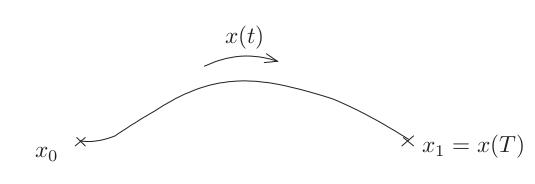
\includegraphics[width=\textwidth]{images/controle.png}
\end{figure}
Si la condition précédente est remplie, existe-t-il un contrôle joignant $\psi_0$ à $\psi_{cible}$ , et qui de plus minimise une certaine fonctionnelle $J(\varepsilon)$ ?
\subsection*{Contrôle optimal}
La fonctionnelle $J(\varepsilon)$ est un critère d’optimisation, on l’appelle le coût . Par exemple ce coût
peut être égal au temps de parcours; dans ce cas c’est le problème du temps minimal.
%Nous voulons construire un contrôle d'amplitude "raisonnable" afin d’amener le système d'un état initial $\psi_0$ à un état cible $O\psi(T)$. 
%$O$ étant l'observable décrivant l'état cible. \\\\
\begin{figure}[h]
	\caption{Problème de contrôle optimal}
	\centering
	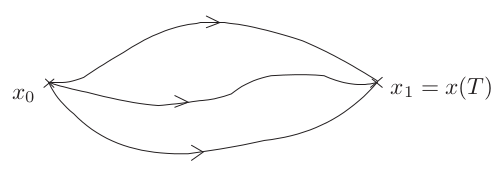
\includegraphics[width=\textwidth]{images/controleoptimal.png}
\end{figure}

On considère ainsi une fonctionnelle $J$
\begin{equation}
J(\varepsilon) = \langle \psi(T)|O|\psi(T) \rangle - \alpha \int_{0}^{T}\varepsilon^2(t)dt \quad \alpha \in \R_+
\end{equation}
et on se pose le problème: Trouver $\varepsilon$ tel que $\varepsilon$ résout
$$ \max_{\varepsilon \in L^2(0,T)} J(\varepsilon)$$
Au maximum de la fonctionnelle $J(\varepsilon)$, les équations de Euler-Lagrange sont satisfaites. Le Lagrangien du système est donné par :
\begin{equation} \label{lagrangien}
L(\psi,\varepsilon,\chi)= J(\varepsilon)\\
-2\Re \bigg\{ \int_{0}^{T}\langle \chi (t)|\partial_{t}+i(H_0+V-\mu(x)\varepsilon(t))|\psi(t) \rangle dt \bigg\}
\end{equation}
\section*{Schémas monotones}
Une stratégie éfficace de résolution de ces équations est donnée par une classe d’algorithmes relevant du contrôle quantique, les schémas monotones. Ils ont étés introduits en 1992 par David Tannor, Vladimir Kazakov et V. Orlov,  \cite{Tannor}, sur la base des travaux de Krotov \cite{Krotov1}, \cite{Krotov2}. Une amélioration a ensuite été proposée par Wusheng Zhu et Herschel Rabitz \cite{Zhu} en 1998. Une généralisation est donnée par Yvon Maday et Gabriel Turinici en 2003 \cite{Maday}.\\\\

Comment construire une discrétisation temporelle puis spaciale de ces algorithmes qui préserve la propriété de monotonie?\\\\

Dans le Chapitre Premier, nous introduisons la mécanique quantique en trois postulats et présentons le cadre général du contrôle quantique. Le Chapitre Deux est dédié aux schémas monotones pour l'équation de Schrödinger.
Différentes discrétisations de ces schémas sont proposées dans le Chapitre Trois.
\newpage
\chapter{Mécanique quantique et contrôle quantique}

\section{La mécanique quantique en trois postulats}
\subsection{Premier postulat de la mécanique quantique}
\subsubsection{Fonction d'onde}
En mécanique quantique, l'état d'un système donné, est donné par son vecteur d'état $|\psi (t)\rangle$. 
%On utilise la notation bra-ket introduite par Dirac \footnote{Paul Dirac, Les Principes de la mécanique quantique [« The Principles of Quantum Mechanics »] (1re éd. 1930) } pour représenter les états quantiques de manière concise et simple. Le vecteur $\psi$ est ainsi noté $|\psi \rangle$ et appelé \textbf{ket}, tandis que son vecteur dual est appelé \textbf{bra} et noté $\langle \psi |$. \\
L'espace des états dépend du système considéré. Par exemple, dans le cas le plus simple où le système n'a pas de spin, les états quantiques sont des fonctions $\psi$ :
$$
\begin{aligned}
	\psi :\quad \quad \mathbb {R} ^{3}&\rightarrow \mathbb{C} \\(x,y,z)&\mapsto \psi (x,y,z)
\end{aligned}
$$
telles que l'intégrale  $\int _{\mathbb{R} ^{3}}|\psi (\mathbf{r} )|^{2}d\mathbf{r}$ converge. Dans ce cas, $\psi$ est appelée la fonction d'onde du système.
\subsubsection{Cas d’une particule dans l’espace à une dimension}
La probabilité pour que la particule soit dans l’intervalle $[a,b]$ est donnée par l’aire de la courbe située entre $x=a$ et $x=b$ (figure si possible)
\begin{equation}
\int_a^b dP(x)= \int_a^b |\psi(x,t)|^2dx
\end{equation}
Il est impossible de connaître avec précision la position de la particule à un instant t. On ne peut que connaître la probabilité $dP(x)$ pour qu’elle soit entre $x$ et $x+dx$, soit:
\begin{equation}
dP(x)=|\psi(x,t)|^2dx=\psi(x,t)\overline{\psi(x,t)}dx
\end{equation}
La particule doit être quelque part sur l’axe $X’OX$, par conséquent:
\begin{equation}
\int_{-\infty}^{+\infty}|\psi(x,t)|^2dx=1
\end{equation}
pour tout $t$. $\psi$ est donc de carré sommable.
La densité de probabilité est donnée par
\begin{equation}
\dfrac{dP(x,t)}{dx}=|\psi(x,t)|^2=\rho(x,t)
\end{equation}

\subsubsection{Cas d’une particule dans l’espace à trois dimensions}
On a 
\begin{equation}
\int dP(\vec{r},t)=\iiint_{espace}|\psi(x,t)|^2d^3r=1
\end{equation}

Où $d^3r$ représente l'élément de volume donnée par: $$d^3r=dxdydz=r^2sin\theta dr d\theta d\varphi$$

\subsubsection{Cas de N particules}
L’espace le mieux adapté à la description des systèmes en physique quantique est un espace $\Omega$, nommé espace des configurations qui représente l’ensemble de toutes les configurations possibles du système. Par exemple, dans le cas d’un système à $N$ particules isolées et sans contraintes, l’espace des configurations est $\Omega = \R^{3N}$ et $\psi(x,t) \in L^2(\Omega, \C)$.

\begin{Post}
	A tout système quantique correspond un espace de Hilbert complexe $\mathcal{H}$, tel que l’ensemble des états accessibles au système soit en bijection avec la sphère unité de $\mathcal{H}$.
\end{Post}

\subsection{Observables et deuxième postulat}
Une observable est l'équivalent en mécanique quantique d'une grandeur physique en mécanique classique, comme la position, la quantité de mouvement, l'énergie, etc. Une observable est formalisée mathématiquement par un opérateur hermitien (endomorphisme autoadjoint) sur $\mathcal{H}$ (chaque état quantique est représenté par un vecteur de $\mathcal{H}$). 
%Cet operateur permet de décomposer un état quantique quelconque $|\psi \rangle$ en une combinaison linéaire d'états propres,
\begin{ex}
	Exemples d'observables
	\begin{enumerate}
		\item la position: $X$
		\item l'énergie potentielle: $V$
		\item la quantité de mouvement: $P=-i\hbar \nabla$
		\item l'énergie cinétique:
		$H_0=\dfrac{P \cdot P}{2m}=-\dfrac{\hbar ^{2}}{2m}\nabla^{2}$
		\item l'énergie totale, appelée hamiltonien:
		$H=H_0+V$
	\end{enumerate}
\end{ex}
%En mécanique quantique, une grandeur ne prend une valeur déterminée que lors d’une mesure:
\begin{Post}
	A toute grandeur physique représentée par l'observable $\mathcal{A}$ correspond un opérateur $A$ auto-adjoint sur $\mathcal{H}$, vérifiant la propriété suivante : le résultat de la mesure d’une grandeur physique $\mathcal{A}$ ne peut être qu’un élément du spectre de $A$.
\end{Post}
Les valeurs propres sont les valeurs pouvant résulter d'une mesure idéale de cette propriété, les vecteurs propres étant l'état quantique du système immédiatement après la mesure et résultant de cette mesure. Ce postulat peut donc s'écrire :
$$
A|\alpha _{n}\rangle =a_{n}|\alpha _{n}\rangle 
$$
où $A$, $|\alpha_{n}\rangle$ et $a_n$ désignent, respectivement, l'observable, le vecteur propre et la valeur propre correspondante.\\
Les états propres de tout observable $A$ forment une base orthonormée dans l'espace de Hilbert $\mathcal{H}$.
Cela signifie que tout vecteur $|\psi (t)\rangle$ peut se décomposer de manière unique sur la base de ces vecteurs propres $|\phi_{i}\rangle$:
$$
|\psi \rangle =c_{1}|\phi _{1}\rangle +c_{2}|\phi _{2}\rangle +...+c_{n}|\phi _{n}\rangle +...
$$
La moyenne des mesures de $\mathcal{A}$ est quant à elle égale à $\langle\psi|A|\psi\rangle$ où la notation $\langle\cdot|A|\cdot\rangle$ est définie par :
\begin{equation}
\langle\psi|A|\chi\rangle = \int_{\Omega} \bar{\psi}A\chi
\end{equation}
%ou $\psi$ et $\chi$ sont des fonctions de $L^2(\Omega, \C)$ et $A$ un opérateur arbitraire défini de $L^2(\Omega, \C)$ dans lui-même.
\begin{ex}
	La position moyenne sur l’axe des abscisses:
	\begin{equation*}
	\langle X \rangle = \int_{- \infty}^{- \infty} x |\psi(x,t)|^2 dx
	\end{equation*}
\end{ex}

\subsection{Equation de Schrödinger et troisième postulat}
L'équation de Schrödinger, proposée par le physicien autrichien Erwin Schrödinger en 1952, est une équation fondamentale en mécanique quantique. Elle décrit l'évolution dans le temps d’une particule massive non relativiste, et remplit ainsi le même rôle que la relation fondamentale de la dynamique en mécanique classique $\dfrac{dp}{dt}=F$.
\begin{Post}
	Entre deux mesures, l’évolution de l’état est régie par l’équation de Schrödinger
	\begin{equation} \label{sch1}
	i\hbar \dfrac{\partial }{\partial t} \psi (x,t) = H\psi (x,t)
	\end{equation}
\end{Post}
%\subsubsection{Exemple de resolution de \eqref{sch1}: cas d'une particule libre}
Considérons le cas d'une particule libre ($V=0$) et menons notre étude sur $\R^m$ $(m \geq 1)$ nous étudions alors l'équation
\begin{equation} \label{chauchy2}
u'(t)=Au(t)
\end{equation}
où $A$ est un opérateur sur $E=L^2(R^m)$ défini par 
$$
Au=ik\Delta u=ik(\partial_{1}^2u+...+\partial_{m}^2u)
$$
$k$ une constante réelle. Le domaine de $A$ est l'ensemble des $u \in L^2(R^m)$ tel que $\Delta u$ (au sens des distributions) appartient à $L^2$.
\begin{definition}
	On dit que le problème de Cauchy pour l'équation \eqref{chauchy2} est bien posé si les deux hypothèses suivantes sont satisfaites:
	\begin{enumerate}
		\item[(a)] \textbf{Existence et unicité de solutions}: Il existe un sous-espace dense $D$ de $E$ tel que, pour tout $u_0 \in D$, il existe une unique solution $u(.)$ de \eqref{chauchy2} avec $u(0)=u_0$
		\item[(b)] \textbf{La solution dépend de façon continue des données} Il existe une fonction non décroissante, non négative $C(t)$ tel que
		$$
		||u(t)||\leq C(t) ||u(0)||
		$$
	\end{enumerate}
\end{definition}
En appliquant la transformée de Fourier à \eqref{chauchy2}, nous obtenons
\begin{align*} 
\mathcal{F}[Au](\xi) &= \mathcal{F}[ik\Delta u](\xi) \\ 
&= ik\mathcal{F}[\Delta u](\xi) \\
&= -ik|\xi|^2 \mathcal{F}[u](\xi) \\
\mathcal{F}[Au](\xi) &= -ik|\xi|^2 \tilde{u}(\xi)
\end{align*}
Alors si $u_0 \in D(A)$ nous obtenons une solution:
\begin{equation}
u(t)=\mathcal{F}^{-1}(exp(-ik|\xi|^2 t)\mathcal{F}[u_0](\xi))
\end{equation}
Puisque $D(A)$ est dense dans $E$, on déduit que \eqref{chauchy2} admet une unique solution sur $E$.\\
Ensuite, observons que si $u \in D(A)$, alors
\begin{align*}
(Au,u) &= (\mathcal{F}[Au],\mathcal{F}[u])\\
&= ik\int|\xi|^2 |\tilde{u}|^2
\end{align*}
Ainsi, $\Re (Au,u)=0$\\
Par conséquent, si $u(.)$ est une solution de \eqref{chauchy2}, nous avons:
\begin{align*}
\partial_{t}||u(t)||^2 &= 2 \Re (u'(t),u(t))\\
&= 2 (Au(t),u(t))\\
&=0
\end{align*}
Ainsi, $||u(t)||$ est constante:
\begin{equation} \label{normecons}
||u(t)||=||u(0)|| \quad \forall t \in \R
\end{equation}
En conclusion, le problème de Cauchy pour \eqref{chauchy2} est bien posé pour tout $t$.\\
En outre, \cite{Fattorini} généralise ce résultat sur $E=L^p (\R^m)$ avec $1 \leq p < m$.

\section{Contrôle quantique}
On rappelle que l'état $\psi(t)$ d'un système quantique évolue conformément à l'équation de Schrödinger:
\begin{equation}
i \hbar \dfrac{\partial }{\partial t} \psi (x,t) = H\psi (x,t),\quad \quad \psi(t=0)=\psi_0
\end{equation}
où $H$ est un endomorphisme auto-adjoint sur $\mathcal{H}$ appelé Hamiltonien interne du système. $\hbar$ est la constante de Planck. Dans la suite, nous travaillons en unités atomiques, c'est-à-dire $\hbar=1$ et l'état initial a une norme unitaire, $||\psi_0||^2 \equiv \langle \psi_0|\psi_0 \rangle =1$.
\subsection{Exemple de modèle bilinéaire (BLM)}
Pour simplifier, nous considérons un système quantique de dimension finie. C'est une approximation appropriée dans de nombreuses situations pratiques. Pour un système quantique de dimension $N$, $\mathcal{H}$ est un espace de Hilbert complexe de dimension $N$. Les valeurs propres $(\phi_{i})_{1 \leq i \leq N}$ de $H$ forment une base orthogonale de $\mathcal{H}$.\\
Dans de nombreuses situations, le contrôle du système peut être réalisé par un ensemble de fonctions de contrôle $\varepsilon_{k}(t) \in \R$ couplées au système via une famille d'opérateurs hermitiens indépendants du temps $\{H_k, k=1,2,...\}$. L'Hamiltonien total $H+\sum_{k} \varepsilon_{k}(t)H_k$ détermine alors la nouvelle dynamique du système.
\begin{equation} \label{schcon}
i \dfrac{\partial }{\partial t} \psi (x,t) = (H+\sum_{k} \varepsilon_{k}(t)H_k)\psi (x,t)
\end{equation}
Le but typique d'un problème de contrôle quantique défini sur le système \eqref{schcon} est de trouver en temps fini $T > 0$ un ensemble de contrôles admissibles $u_k(t) \in \R$ qui conduit le système d'un état initial $\psi_0$ à un état prescrit $\psi_{cible}$.
\subsection{Cas d'un champs laser}
En vue de modéliser les interactions onde-matière à l'échelle atomique, nous introduisons un contrôle, généré par un dipôle électrostatique de moment dipolaire $\mu (x)$, émettant un champs (électrique) laser, d'amplitude $\varepsilon (t)$ dépendant du temps.\\
La dynamique du système est désormais donnée par:
\begin{equation} \label{schcon2}
\begin{cases}
i \dfrac{\partial }{\partial t} \psi (x,t) &= H\psi (x,t)-\mu(x)\varepsilon(t)\psi (x,t) \\
\psi (x,t=0) &= \psi_0(x)
\end{cases}
\end{equation}

\section{Discrétisation temporelle}
Choisissons deux paramètres de discrétisation temporelle $N$ et $\Delta T$ tels que $N \Delta T = T$ et notons $\psi_j$ l'approximation de $\psi(j\Delta T)$, $0 \leq j \leq N$.
\subsection{Méthode du splitting d’opérateur}
Considérons l’équation différentielle ordinaire scalaire
\begin{equation} \label{edo1}
\dot{x}=(a+b)x, \quad \quad x(0)=x_0
\end{equation}
où $a$ et $b$ sont des scalaires. On connaît la solution exacte de cette equation :
\begin{align*}
x(t)=exp((a+b)t)x_0 &= exp(at)exp(bt)x_0 \quad \mbox{(methode 1)}\\
&= exp(bt)exp(at)x_0 \quad \mbox{(methode 2)}
\end{align*}
Nous pouvons ainsi séparer l'évolution selon \eqref{edo1} en deux temps :
$$\mbox{(L1)}
\begin{cases}
\dot{y}=by,\quad y(0)=x_0\\
\dot{x}=ax,\quad x(0)=y(t)
\end{cases}
$$
$$\mbox{(L2)}
\begin{cases}
\dot{y}=ay,\quad y(0)=x_0\\
\dot{x}=bx,\quad x(0)=y(t)
\end{cases}
$$
Pour le système (L1), on a clairement
\begin{align*}
x(t) &= exp(at)x_0\\
&= exp(at)y(t)\\
&= exp(at)exp(bt)y(0)\\
&= exp(at)exp(bt)x_0
\end{align*}
Pour (L2), le calcul se fait de la même manière et donne le même résultat.\\\\
On appelle \textbf{splitting de Lie} ou méthode à pas fractionnaire les deux méthodes (L1) et (L2). Pour une equation scalaire, ces deux méthodes sont identiques et reviennent au même que de traiter l’équation en une seule fois.
Pour exprimer le splitting dans notre exemple, nous avons été obligés d’introduire une variable intermédiaire $y$. Ceci s’avérerait à l’usage peu pratique pour des contextes plus compliqués. Nous introduisons donc les semi-groupes.
\begin{definition}
Soit $X$ un espace de Banach. Une famille $(T(t))_{t \geq 0}$ d'opérateurs linéaires bornés de $X$ dans $X$ est un semi-groupe fortement continu d'opérateurs linéaires bornés si
\begin{enumerate}
	\item[(i)] $T(0)=id_X$;
	\item[(ii)] $T(t+s)=T(t)T(s), \: \forall t, s \geq 0$;
	\item[(iii)] $\forall x \in X, \:\: \R \ni t \mapsto T(t)x \in X$ est continue en $0$.  
\end{enumerate}
\end{definition}
\begin{remark}
	Un semi-groupe d'opérateurs linéaires bornés $(T(t))_{t\geq 0}$, est uniformément continu si
	$$
	\lim_{t \rightarrow 0} ||T(t)-I||=0
	$$
\end{remark}
Un semi-groupe fortement continu d'opérateurs linéaires bornés sur $X$ sera appelé semi-groupe de classe $C_0$ ou simplement $C_0$ semi-groupe.\\

Si seulement (i) et (ii) sont satisfaits, on dit que la famille $(T(t))_{t\geq 0}$ est un semi-groupe.
\begin{definition}
	L'opérateur linéaire $A$ défini par
	\begin{equation}
	D(A)= \left \{ x \in X : \lim_{t \rightarrow 0^+} \dfrac{T(t)x-x}{t} \mbox{ existe} \right \}
	\end{equation}
	et
	\begin{equation}
	Ax=\lim_{t \rightarrow 0^+} \dfrac{T(t)x-x}{t} \quad \mbox{pour } x \in D(A)
	\end{equation}
	est le générateur infinitésimal du semi-groupe $(T(t))_{t\geq 0}$; $D(A)$ est le domaine de $A$
\end{definition}
\subsubsection{Splittings de Strang}
L’application qui à $x_0$ associe $x(t)$ par le flot de l’EDO est le semi-groupe que nous noterons $S(t)$
\begin{equation}
x(t)=S(t)x_0=exp((a+b)t)x_0
\end{equation}
On note $A(t)$ et $B(t)$ les semi-groupes associés aux deux parties de l’équation, à savoir
$$
A(t)x_0=exp(at)x_0, \quad \quad B(t)x_0=exp(bt)x_0
$$
Les deux splittings de Lie (L1) et (L2) consistent donc à écrire
$$
\mbox{\textbf{(L1)}: } x(t)=A(t)B(t)x_0, \quad \quad \mbox{\textbf{(L2)}: } x(t)=B(t)A(t)x_0
$$
On definit sans effort deux nouveaux types de splitting : les \textbf{splittings de Strang} \cite{Strang}
$$
\mbox{\textbf{(S1)}: } x(t)=A(\dfrac{t}{2})B(t)A(\dfrac{t}{2})x_0, \quad \quad \mbox{\textbf{(S2)}: } x(t)=B(\dfrac{t}{2})A(t)B(\dfrac{t}{2})x_0
$$
Les méthodes de Lie et de Strang sont respectivement d’ordre 1 et 2.
\subsubsection{Splitting de Strang pour l'équation de Schrödinger}
Afin de présenter le schéma de splitting, on considère un problème d'évolution général. Soit $A$ et $B$, deux opérateurs auto-adjoints, tels que : $D(A) \subset \mathcal{H}$, $D(B) \subset \mathcal{H}$ et $A+B$ est un opérateur auto-adjoint sur $D(A) \cap D(B)$. On note ici $D(A)$ et $D(B)$ les domaines respectifs des opérateurs $A$ et $B$. Considérons le problème d'évolution
\begin{equation}
\begin{cases}
i \partial_t \psi (x,t) &= A\psi (x,t)+B\psi (x,t), \quad x \in \Omega, t>0 \\
\psi (x,t=0) &= \psi_0(x) \in \mathcal{H}
\end{cases}
\end{equation}
et notons $\psi(x,t)=e^{-i(A+B)t}\psi_0(x)$ sa solution pour $t>0$, et $x\in \Omega$. Le schéma de splitting consiste à approcher la solution $\psi$ du problème d'évolution via une approximation de l'opérateur $e^{-i(A+B)t}$ à travers les opérateurs $e^{-iA}$ et $e^{-iA}$. Ceci permet alors d'avoir à résoudre successivement deux equations plus simples. 
\\Ici, $A=H_0$ et $B=V(x)-\mu(x)\varepsilon(t)$ est la partie potentielle. On obtient l'approximation
\begin{equation}
\psi(x,t+\Delta T) \approx e^{-iH_0 \frac{\Delta T}{2}}e^{-i(V(x)-\mu\varepsilon)\Delta T}e^{-iH_0 \frac{\Delta T}{2}} \psi(x,t)
\end{equation}
\begin{pro}
	Cette méthode conserve la norme $L^2$ de la fonction d’onde $\psi$ au cours du temps.
\end{pro}
\begin{ proof }
	Les opérateurs exponentiés étant antihermitiens, leurs exponentielles sont unitaires. En effet, notons $X^{T}$, $\overline{X}$ et $X^{\dagger}=(\overline{X})^T$ respectivement la transposée, la conjuguée et l'adjointe de $X$. Puisque $e^{X^T}={(e^X)}^T$ et $e^{\overline{X}}=\overline{e^X}$ alors ${e^X}^{\dagger}={(e^X)}^{\dagger}$. Il s'ensuit que si X est antihermitienne, c'est-à-dire $X^{\dagger}=-X$, alors ${(e^X)}^{-1}={(e^X)}^{\dagger}$ : $e^X$ est unitaire.
\end{ proof }
Cette propriété importante \eqref{normecons} est donc conservée après discrétisation.\\
D’autres méthodes de résolution approchée peuvent être envisagées : schémas d’Euler, Runge-Kutta... Le problème posé par ces schémas est qu’ils ne conservent pas la norme de la solution en général.
\subsection{Schéma de Cranck-Nicholson}
Une exception existe avec le schéma implicite de Cranck-Nicholson défini dans notre cas par :
\begin{equation}
i\dfrac{\psi_{j+1}-\psi_j}{\Delta T}=(H_0-\mu\varepsilon_j)\dfrac{\psi_{j+1}+\psi_j}{2}
\end{equation}
En tant que schéma implicite, son inconvénient majeur est d’être coûteux.
\chapter{Schémas monotones pour l'équation de Schrödinger}

\section{Introduction}

Considérons un système quantique décrit par une fonction d’onde $\psi(x, t)$ soumis à un champ électrique $\varepsilon(t)$ et dont l’état initial $\psi(x, 0) = \psi_0 (x)$ est supposé connu. Comme stipulé au \eqref{schcon2}, l’évolution d’un tel système est régie par l’équation:

\begin{equation}
\begin{cases}
i \frac{\partial}{\partial t} \psi (x,t) = H\psi(x,t) - \mu(x)\varepsilon(t)\psi(x,t)\\
\psi(x,t=0)=\psi_0(x)
\end{cases}
\end{equation}

Le moment dipolaire $\mu$ est supposé connu et indépendant du temps.

\section{Fonctionnelles de coût}
Soit $\alpha : [0, T ] \longrightarrow \R^+$ une fonction bornée, $O$ un opérateur symétrique borné, $T$ un réel positif, $\varepsilon$ une fonction de $L^2 ([0, T ], \R),\  \psi : \Omega \times [0, T ] \longrightarrow \C$ une fonction d’onde dépendant du temps et $\psi_{cible} : \Omega \longrightarrow C$ une fonction d’onde fixée.
\\Nous considerons deux fonctionnelles de coût:

\begin{equation}
J_1(\varepsilon) = \langle \psi(T)|O|\psi(T) \rangle - \int_0^T \alpha(t)\varepsilon^2(t)dt
\end{equation}

\begin{equation}
J_2(\varepsilon) = 2\Re\langle \psi_{cible}|\psi(T)\rangle - \int_0^T \alpha(t)\varepsilon^2(t)dt
\end{equation}

$\psi_{cible}$ représente une fonction d’onde cible. $J_1$ releve du formalisme attaché aux observables tandis que $J_2$ est plus simple a manipuler.
%Les deux permettent de réaliser un compromis entre la recherche d'une grande valeur de l’observable et une norme $L_2$ du champ $\varepsilon$ raisonnable.
Le maximum du terme $2\Re\langle \psi_{cible}|\psi(T)\rangle$ est bien atteint pour $\psi(T) = \psi_{cible}$ puisque $\lVert \psi_{cible} \rVert = 1$ et que $2\Re\langle \psi_{cible}|\psi(T)\rangle = -\lVert \psi_{cible} - \psi(T)\rVert ^2+2$.

\begin{remark}

Les opérateurs, tels que $O$, associés à des observables sont toujours supposés bornés sur $L^2 ([0, T ], \R)$ dans cette thèse. Sans perte de généralité, il est de plus possible de les considérer comme définis positifs. Par exemple, en notant $\lVert O \rVert_*$ la norme de l'opérateur $O$, l’opérateur $\tilde{O} = O + 2\lVert O \rVert_* Id$ est défini positif. Le remplacement de O par $\tilde{O}$ n’entraîne qu'un décalage de $ 2 \lVert O \rVert_*$ de la valeur de la fonctionnelle, puisqu'une fonction d'onde est toujours de norme égale à $1$ dans $L^2 (\Omega)$. Les maxima de $J$ ne sont donc pas affectés par cette modification sur $O$.

\end{remark}

D’un point de vue algébrique, le multiplicateur de Lagrange est le même que celui introduit au paragraphe 1.5.2, à un facteur $\frac{1}{2} $ près. Ce choix est effectué pour des raisons pratiques puisque des simplifications sont alors possibles grâce à la présence de termes quadratiques dans les fonctionnelles $J_1$ et $J_2$ définies par les équations (1.14) et (1.15). Les équations d'Euler-Lagrange sont alors données pour $J_1$ par :

\begin{equation}
\begin{cases}
i \frac{\partial}{\partial t} \psi (x,t) = H - \varepsilon(t)\mu(x)\psi(x,t)\\
\psi(x,t=0)=\psi_0(x)
\end{cases}
\end{equation}

\begin{equation}
\begin{cases}
i \frac{\partial}{\partial t} \chi (x,t) = H - \varepsilon(t)\mu(x)\chi(x,t)\\
\chi(x,t=T)=O\psi(x,T)
\end{cases}
\end{equation}

\begin{equation}
\alpha(t)\varepsilon(t) = -\Im \langle \chi(t)|\mu|\psi(t)\rangle 
\end{equation}

et pour $J_2$ par:

\begin{equation}
\begin{cases}
i \frac{\partial}{\partial t} \psi (x,t) = H - \varepsilon(t)\mu(x)\psi(x,t)\\
\psi(x,t=0)=\psi_0(x)
\end{cases}
\end{equation}

\begin{equation}
\begin{cases}
i \frac{\partial}{\partial t} \chi (x,t) = H - \varepsilon(t)\mu(x)\chi(x,t)\\
\chi(x,t=T)=\psi_{cible}(x)
\end{cases}
\end{equation}

\begin{equation}
\alpha(t)\varepsilon(t) = -\Im \langle \chi(t)|\mu|\psi(t)\rangle 
\end{equation}

Notons de plus que dans ces deux fonctionnelles, seule la valeur au temps T des fonctions d’onde est prise en compte. Les résultats exposés dans ce mémoire peuvent s'appliquer cependant dans certains cas à des fonctionnelles comportant des termes de la forme :

\begin{equation}
\int_0^T \langle \psi(t)|O'(t)|\psi(t)\rangle + \lambda \Re\langle \psi_{ref}(t)|\psi(t)\rangle dt
\end{equation}

où $O'(t)$ et $\psi_{ref}(t)$ représentent respectivement une observable et une fonction d'onde dépendant du temps. Signalons enfin que l'existence de maxima de $J_1$ et de $J_2$ et de fonctionnelles plus générales a été montrée dans [30] et [31].

\section{Schémas monotones}
Supposons $\varepsilon_k$ connu et voyons comment déterminer $\tilde{\varepsilon}^k$ et $\varepsilon^{k+1}$ , les champs permettant le calcul des propagations respectives de $\chi^k$ et $\psi^{k+1}$ . Les formules des accroissements (1.11), (1.12) donnent dans les cas des fonctionnelles $J_1$ et $J_2$ :

\begin{equation}
\begin{split}
J_1(\varepsilon^{k+1} - J_1(\varepsilon^k) = \int_0^T (\tilde{\varepsilon}^k(t) - \varepsilon^{k+1}(t))(2\Im\langle \chi^k(t)|\mu|\psi^{k+1}(t)\rangle + \alpha(t)(\tilde{\varepsilon}^k(t) + \varepsilon^{k+1}(t)))dt \\
+ \int_0^T(\varepsilon^k(t) - \tilde{\varepsilon}^k(t))(2\Im\langle \chi^k(t)|\mu|\psi^k(t)\rangle + \alpha(t)(\varepsilon^k(t) + \tilde{\varepsilon}^k(t)))dt \quad\\
+ \langle \delta \psi^{k+1,k}(T)|O|\delta\psi^{k+1,k}(T)\rangle dt \phantom{111111111111111111111111111111}
\end{split}
\end{equation}

\begin{equation}
\begin{split}
J_2(\varepsilon^{k+1} - J_2(\varepsilon^k) = \int_0^T (\tilde{\varepsilon}^k(t) - \varepsilon^{k+1}(t))(2\Im\langle \chi^k(t)|\mu|\psi^{k+1}(t)\rangle + \alpha(t)(\tilde{\varepsilon}^k(t) + \varepsilon^{k+1}(t)))dt \\
+ \int_0^T(\varepsilon^k(t) - \tilde{\varepsilon}^k(t))(2\Im\langle \chi^k(t)|\mu|\psi^k(t)\rangle + \alpha(t)(\varepsilon^k(t) + \tilde{\varepsilon}^k(t)))dt \quad
\end{split}
\end{equation}

Notons $I_k$ la partie intégrale commune à ces deux formules.

\begin{equation}
\begin{split}
I_k = \int_0^T (\tilde{\varepsilon}^k(t) - \varepsilon^{k+1}(t))(2\Im\langle \chi^k(t)|\mu|\psi^{k+1}(t)\rangle + \alpha(t)(\tilde{\varepsilon}^k(t) + \tilde{\varepsilon}^{k+1}(t)))dt \\
+ \int_0^T(\varepsilon^k(t) - \tilde{\varepsilon}^k(t))(2\Im\langle \chi^k(t)|\mu|\psi^k(t)\rangle + \alpha(t)(\varepsilon^k(t) + \tilde{\varepsilon}^k(t)))dt \quad
\end{split}
\end{equation}

Des conditions suffisantes pour assurer la monotonie de la suite $(J(\varepsilon^k))_{k \in \N}$ sont alors données par le critère $(C)$ suivant :

\begin{equation*}
\forall t \in [0,T],\ 
\begin{cases}
\quad(\varepsilon^k(t) - \tilde{\varepsilon}^k(t))(2\Im\langle \chi^k(t)|\mu|\psi^k(t)\rangle + \alpha(t)(\varepsilon^k(t) + \tilde{\varepsilon}^k(t))) \quad \quad \quad \geq 0\\
\phantom{11111111111111111111111111111111111111111111111111111111}\quad \quad \quad(C) \\
(\tilde{\varepsilon}^k(t) - \varepsilon^{k+1}(t))(2\Im\langle \chi^k(t)|\mu|\psi^{k+1}(t)\rangle + \alpha(t)(\tilde{\varepsilon}^k(t) + \varepsilon^{k+1}(t))) \quad \geq 0
\end{cases}
\end{equation*}

Nous passons en revue dans les sections suivantes différentes approches permettant d’assurer la vérification du critère $(C)$.

\paragraph*{Monotonie imposée par une condition algébrique}
$ $\\
Remarquons que $I_k$ peut être écrit sous la forme suivante :

\begin{align}
I_k & = \int_0^T \alpha(t)\left[ \left(\varepsilon^{k+1}(t) + \frac{1}{\alpha(t)} \Im\langle \chi^k(t)|\mu|\psi^{k+1}(t)\rangle \right)^2 - \left(\tilde{\varepsilon}^k(t) + \frac{1}{\alpha(t)} \Im\langle \chi^k(t)|\mu|\psi^{k+1}(t)\rangle \right)^2 \right] dt \\
& \quad \quad \quad + \int_0^T \alpha(t)\left[ \left(\tilde{\varepsilon}^k(t) + \frac{1}{\alpha(t)} \Im\langle \chi^k(t)|\mu|\psi^k(t)\rangle \right)^2 - \left(\varepsilon^k(t) + \frac{1}{\alpha(t)} \Im\langle \chi^k(t)|\mu|\psi^k(t)\rangle
 \right)^2 \right] dt
\end{align}

Cette expression permet de formuler une condition algébrique ([32]) assurant la positivité de l'accroissement. La détermination de $\tilde{\epsilon}^k$ est effectuée à partir de $ \epsilon^k$ sous le critère imposé par le terme (1.19) :

$$\forall t \in [0,T],\ \left|\tilde{\varepsilon}^k(t) + \frac{1}{\alpha(t)} \Im\langle \chi^k(t)|\mu|\psi^k(t)\rangle\right|\leq \left|\varepsilon^k(t) + \frac{1}{\alpha(t)} \Im\langle \chi^k(t)|\mu|\psi^k(t)\rangle\right| $$

tandis que $\varepsilon^{k+1}$ est déterminé à partir de $\tilde{\varepsilon}^k$ sous le critère imposé par le terme (1.18) :

$$\forall t \in [0,T],\ \left|\varepsilon^{k+1}(t) + \frac{1}{\alpha(t)} \Im\langle \chi^k(t)|\mu|\psi^{k+1}(t)\rangle\right|\leq \left|\varepsilon^k(t) + \frac{1}{\alpha(t)} \Im\langle \chi^k(t)|\mu|\psi^{k+1}(t)\rangle\right| $$

La figure 1.2 illustre le critère issu de (1.19). L'avantage de cette formulation est qu'elle laisse une liberté de choix relative sur les caractéristiques des champs obtenus. Le champ peut par exemple être astreint à être borné ou encore à prendre ses valeurs dans un ensemble discret. Définissons par exemple les fonctions $sign^+$ et $sat_M$ par :

\begin{equation}
sign^+(x) = \begin{cases}
-1 \quad,\ x< 0\\
\quad 1 \quad,\ x \geq 0
\end{cases}
\end{equation}

\begin{equation}
sat_M(x) = \begin{cases}
-M \quad,\ x\geq -M\\
\quad x\quad,\ -M\geq x \geq M\\
\quad M \quad,\ x\geq M 
\end{cases}
\end{equation}

\noindent et posons alors:
\begin{equation}
\begin{cases}
\tilde{\varepsilon}^k(t) = Msign^+ \left(-\frac{1}{\alpha(t)} \Im\langle \chi^k(t)|\mu|\psi^k(t)\rangle\right)\\
\varepsilon^{k+1}(t) = Msign^+ \left(-\frac{1}{\alpha(t)} \Im\langle \chi^k(t)|\mu|\psi^{k+1}(t)\rangle\right)
\end{cases}
\end{equation}

\noindent qui assure que les champs obtenus ne prennent comme valeurs que $M$ et $-M$ , ou bien

\begin{equation}
\begin{cases}
\tilde{\varepsilon}^k(t) = sat_M \left(-\frac{1}{\alpha(t)} \Im\langle \chi^k(t)|\mu|\psi^k(t)\rangle\right)\\
\varepsilon^{k+1}(t) = sat_M \left(-\frac{1}{\alpha(t)} \Im\langle \chi^k(t)|\mu|\psi^{k+1}(t)\rangle\right)
\end{cases}
\end{equation}

qui contraint les champs à prendre leurs valeurs dans l'intervalle $[-M, M ]$. Les définitions (1.20) et (1.21) conduisent à des schémas monotones.
\\Cette approche se prête particulièrement bien à un couplage avec la méthode du \textit{toolkit} [13] présentée au paragraphe 1.3.3 qui suggère de discrétiser les valeurs du champ pour calculer rapidement les propagations. Les différents schémas présentés dans ce paragraphe donnent en effet lieu à des champs bornés par des constantes arbitraires, voire à des champs prenant un nombre fini de valeurs.

\paragraph*{Schémas monotones à deux paramètres}
$ $\\Dans un article récent [29], Y. Maday et G. Turinici montrent comment assurer la positivité des deux accroissements précédents. L’algorithme proposé prescrit les formules suivantes pour calculer$\tilde{\varepsilon}^k$ et $\varepsilon^{k+1}$ :

\begin{equation}
\begin{split}
\tilde{\varepsilon}^k(t) = (1-\eta)\varepsilon^k(t)-\frac{\eta}{\alpha(t)} \Im\langle \chi^k(t)|\mu|\psi^k(t)\rangle\quad \\
\varepsilon^{k+1}(t) = (1-\delta)\tilde{\varepsilon}^k(t) -\frac{\delta}{\alpha(t)} \Im\langle \chi^k(t)|\mu|\psi^{k+1}(t)\rangle
\end{split}
\end{equation}

où $\delta$ et $\eta$ peuvent être arbitrairement choisis dans $[0, 2]$. En reportant ces deux définitions dans les accroissements (1.16) et (1.17), ceux-ci s’écrivent alors sous la forme :
\begin{align*}
J_1(\varepsilon^{k+1})-J_1(\epsilon^k) &= \langle \psi^{k+1}(T) - \psi^k(T)|O|\psi^{k+1}(T) - \psi^k(T)\rangle\\
\quad & + \int_0^T \alpha(t)(\frac{2}{\delta} - 1)(\varepsilon^{k+1}(t) - \tilde{\varepsilon}^k(t))^2dt\\
 \quad & + \int_0^T \alpha(t)(\frac{2}{\eta} - 1)(\tilde{\varepsilon}^k(t) - \tilde{\varepsilon}^k(t))^2dt
\end{align*}

\begin{align*}
J_2(\varepsilon^{k+1})-J_2(\epsilon^k) &=  \int_0^T \alpha(t)(\frac{2}{\delta} - 1)(\varepsilon^{k+1}(t) - \tilde{\varepsilon}^k(t))^2dt\\
 \quad & + \int_0^T \alpha(t)(\frac{2}{\eta} - 1)(\tilde{\varepsilon}^k(t) - \tilde{\varepsilon}^k(t))^2dt
\end{align*}

Cette formule est valable dans les cas où $\delta$ et $\eta$ ne sont pas nuls. Dans le cas contraire, un calcul analogue montre que la différence reste positive. Une formulation plus générale montre que ce calcul reste valable lorsque les coefficients $\delta$ et $\varepsilon$ dépendent du temps.
L'accroissement obtenu est alors positif ou nul. La monotonie est donc assurée, dès lors que les assignations (1.22) sont effectuées.
\\Signalons enfin que le schéma de Krotov (présenté par Tannor dans [27]) correspond au cas où $(\delta,\eta)= (1, 0)$ tandis que celui de Zhu et Rabitz [28] correspond au cas où $(\delta,\eta)= (1, 1)$.


\chapter{Schémas monotones discrets}

\section{Introduction}
Nous considérons la fonctionnelles :

\begin{equation}
J_1(\varepsilon) = \langle \psi(T)|O|\psi(T) \rangle - \alpha \int_0^T \varepsilon^2(t)dt
\end{equation}
Pour les simulations numériques, nous considérons
\begin{equation}
J_2(\varepsilon) = 2\Re\langle \psi_{cible}|\psi(T)\rangle - \alpha \int_0^T \varepsilon^2(t)dt
\end{equation}

Rappelons que l'opérateur $O$ est défini positif et que $\psi_{cible}$ représente une fonction de $L_2(\Omega,\C)$ de norme $1$, où $\Omega$ est l'espace des configurations. Rappelons également que les équations d'Euler-Lagrange associées à ces fonctionnelles sont dans le cas de $J_1$ :

\begin{equation}
\begin{cases}
i \frac{\partial}{\partial t} \psi (x,t) = (H - \varepsilon(t)\mu(x))\psi(x,t)\\
\psi(x,t=0)=\psi_0(x)
\end{cases}
\end{equation}

\begin{equation}
\begin{cases}
i \frac{\partial}{\partial t} \chi (x,t) = (H - \varepsilon(t)\mu(x))\chi(x,t)\\
\chi(x,t=T)=O\psi(x,T)
\end{cases}
\end{equation}

\begin{equation}
\alpha\varepsilon(t) = -\Im \langle \chi(t)|\mu|\psi(t)\rangle 
\end{equation}

et dans le cas de $J_2$ par:

\begin{equation}
\begin{cases}
i \frac{\partial}{\partial t} \psi (x,t) = (H - \varepsilon(t)\mu(x))\psi(x,t)\\
\psi(x,t=0)=\psi_0(x)
\end{cases}
\end{equation}

\begin{equation}
\begin{cases}
i \frac{\partial}{\partial t} \chi (x,t) = (H - \varepsilon(t)\mu(x))\chi(x,t)\\
\chi(x,t=T)=\psi_{cible}(x)
\end{cases}
\end{equation}

\begin{equation}
\alpha\varepsilon(t) = -\Im \langle \chi(t)|\mu|\psi(t)\rangle 
\end{equation}

où:
\begin{itemize}
	\item $\psi(x, t)$ est la fonction d'onde du système contrôlé,
	\item H est l'Hamiltonien interne associé au système,
	\item $\mu(x)$ est le moment dipolaire, caractéristique lui aussi du système traité. L'opérateur $\mu$ est donc une fonction de $L^2(\Omega, \R)$ que nous identifions avec l'opérateur associé : $\psi \mapsto \mu\psi$,
	\item $\varepsilon(t)$ est le terme de contrôle, soit, dans les cas qui nous intéressent, un champ
	électrique.
\end{itemize}

Sans perte de généralité supposons que l’Hamiltonien s'écrit sous la forme usuelle :
$$ H = H_0+V(x)$$

où $H_0$ est l'opérateur $-\Delta$, opposé du Laplacien et $V(x)$ est le potentiel électrostatique interne.\\

Notons $(\psi_j)_{j = 0\cdots N}, (\chi_j)_{j = 0\cdots N}, (\varepsilon_j)_{j = 0\cdots N-1}, $ et $(\tilde{\varepsilon}_j)_{j = 0\cdots N-1}$ les différentes grandeurs discrétisées à un pas de temps $\Delta T$ . Les discrétisations des deux fonctionnelles conduisent à :

\begin{equation}
J_{\Delta T,1}(\varepsilon) = \langle \psi(T)|O|\psi(T)\rangle - \alpha \Delta T \sum_{j=0}^{N -1} \varepsilon_j^2
\end{equation}

\begin{equation}
J_{\Delta T,2}(\varepsilon) = 2\Re \langle \psi_{cible}|\psi(T)\rangle - \alpha \Delta T \sum_{j=0}^{N -1} \varepsilon_j^2
\end{equation}

Les propagations sont effectuées suivant les formules de splitting d'opérateur présentées au Chapitre Un :

\begin{equation}
\chi_j(x) = e^{iH_0\frac{\Delta T}{2}} e^{i(V(x)-\mu(x)\tilde{\varepsilon}_j)\Delta T} e^{iH_0\frac{\Delta T}{2}} \chi_{j+1}(x)
\end{equation}

avec la condition $\chi_N = O\psi_N$ dans le cas de $J_{\Delta T,1}$ et $\chi_N = \psi_{cible}$ dans le cas de $J_{\Delta T,2}$ et

\begin{equation}
\psi_{j+1}(x) = e^{-iH_0\frac{\Delta T}{2}} e^{-i(V(x)-\mu(x)\varepsilon_j)\Delta T} e^{-iH_0\frac{\Delta T}{2}} \psi_j(x)
\end{equation}

avec un état initial $\psi_0$ fixé.

\section{Calcul de variation}
Nous reprenons le calcul de variation effectue au Chapitre Deux avec nos fonctionnelles discretes
\begin{align*}
J_{\Delta T}(\varepsilon')-J_{\Delta T}(\varepsilon) &= \langle \psi'_N-\psi_N |O|\psi'_N-\psi_N \rangle + 2\Re \langle \psi'_N-\psi_N |O|\psi_N \rangle\\
&\quad +\alpha \Delta T (\sum_{j=0}^{N -1} \varepsilon_j^2-{\varepsilon'}_j^{2})
\end{align*}
Etudions le terme $\langle \psi'_N-\psi_N |O|\psi_N \rangle$ nous obtenons:
\begin{align*}
\langle \psi'_N-\psi_N |O|\psi_N \rangle &= \langle \psi'_N-\psi_N , \chi_N \rangle\\
&=\sum_{j=0}^{N-1} \langle \psi'_{j+1}-\psi_{j+1} , \chi_{j+1}-\chi_{j} \rangle\\
&\quad + \sum_{j=0}^{N-1} \langle \psi'_{j+1}-\psi_{j+1}-\psi_{j+1}+\psi_{j}, \chi_{j} \rangle\\
&=\sum_{j=0}^{N-1} \langle \psi'_{j+1}-\psi_{j+1} , (e^{\frac{H_0\Delta T}{2i}} e^{\frac{V-\mu\tilde{\varepsilon}_j}{i}} e^{\frac{H_0\Delta T}{2i}}-1)\chi_{j} \rangle\\
&\quad + \sum_{j=0}^{N-1} \langle (1-e^{-\frac{H_0\Delta T}{2i}} e^{\frac{-V+\mu\tilde{\varepsilon}_j}{i}} e^{-\frac{H_0\Delta T}{2i}}) \psi'_{j+1}, \chi_{j} \rangle\\
&\quad + \sum_{j=0}^{N-1} \langle (1-e^{-\frac{H_0\Delta T}{2i}} e^{\frac{-V+\mu\tilde{\varepsilon}_j}{i}} e^{-\frac{H_0\Delta T}{2i}}) \psi_{j+1}, \chi_{j} \rangle\\
\end{align*}

Posons alors:

\begin{equation}
\tilde{\psi_j} = e^{-\frac{H_0 \Delta T}{2i}} \psi_j=e^{iH_0 \frac{\Delta T}{2}} \psi_j
\end{equation}
\begin{equation}
\breve{\psi_j} =e^{\frac{H_0 \Delta T}{2i}} \psi_j= e^{-iH_0 \frac{\Delta T}{2}} \psi_j
\end{equation}
\begin{equation}
\breve{\chi_j} =e^{-\frac{H_0 \Delta T}{2i}}\chi_j= e^{iH_0 \frac{\Delta T}{2}} \chi_j
\end{equation}
et
\begin{equation}
\tilde{\chi_j} = e^{\frac{H_0 \Delta T}{2i}}\chi_j= e^{-iH_0 \frac{\Delta T}{2}} \chi_j
\end{equation}
Par suite:
\begin{align*}
\langle \psi'_N-\psi_N |O|\psi_N \rangle &= \sum_{j=0}^{N-1} \langle (e^{\frac{\mu(\tilde{\varepsilon}_j-\varepsilon'_j)}{i}\Delta T}-1)\breve{\psi'_j} , \tilde{\chi_j} \rangle\\
&\quad +\sum_{j=0}^{N-1} \langle \tilde{\psi_{j+1}} (e^{\frac{\mu(\tilde{\varepsilon}_j-\varepsilon_j)}{i}\Delta T}-1)\breve{\chi_{j+1}} \rangle
\end{align*}

Le terme $(e^{\frac{\mu(\tilde{\varepsilon}_j-\varepsilon'_j)}{i}\Delta T}-1)$ nous invite a definir:
\begin{equation} \label{mustar}
\begin{aligned}
\mu^* :\quad \quad \R \times \R &\rightarrow L^2(\Omega, \R) \\(x,y)&\mapsto i\dfrac{e^{\frac{\mu (x-y)}{i}\Delta T }-Id}{\Delta T (x-y)}
\end{aligned}
\end{equation}
On a aussi
\begin{equation*}
\mu^*(x,y)=\dfrac{e^{-i\mu (x-y)\Delta T }-Id}{-i(x-y)\Delta T}
\end{equation*}
D'autre part, on pose:
\begin{equation}
\begin{cases}
a_j(x,y) &=-\frac{1}{\alpha} \Im \langle \tilde{\chi_j}|\mu^*(x,y)|\breve{\psi'_j} \rangle \\
b_j(x,y) &= -\frac{1}{\alpha} \Im \langle \breve{\chi_j}|\mu^*(x,y)|\tilde{\psi_j} \rangle
\end{cases}
\end{equation}
Nous avons:
\begin{align*}
\Re \langle \psi'_N-\psi_N |O|\psi_N \rangle = \alpha \Delta T &\sum_{j=0}^{N-1} a_j (\tilde{\varepsilon}_j,\varepsilon'_j)(\varepsilon'_j- \tilde{\varepsilon}_j)\\
&\quad +b_{j+1} (\varepsilon_j,\tilde{\varepsilon}_j)(\tilde{\varepsilon}_j-\varepsilon_j)
\end{align*}
Nous obtenons ainsi
\begin{align*}
J_{\Delta T}(\varepsilon')-J_{\Delta T}(\varepsilon) &= \langle \psi'_N-\psi_N |O|\psi'_N-\psi_N \rangle \\
&\quad +\alpha \Delta T \sum_{j=0}^{N -1}[(\tilde{\varepsilon}_j-a_j(\tilde{\varepsilon}_j,\varepsilon'_j))^2 - (\varepsilon'_j-a_j(\tilde{\varepsilon}_j,\varepsilon'_j))^2\\
&\quad + (\varepsilon_j-b_{j+1}(\varepsilon_j,\tilde{\varepsilon}_j))^2 - (\tilde{\varepsilon}_j-b_{j+1}(\varepsilon_j,\tilde{\varepsilon}_j))^2]
\end{align*}
Cette formule nous aidera à concevoir des schémas qui restent monotones après la discrétisation dans le temps. En effet, une partie négative des composantes de chaque somme apparaît explicitement. Annuler ou minimiser ces termes nous permettra de concevoir des schémas monotones. \\
Posons donc
\begin{equation}
\phi_j(\tilde{\varepsilon}_j,\varepsilon'_j) = (\tilde{\varepsilon}_j-a_j(\tilde{\varepsilon}_j,\varepsilon'_j))^2 - (\varepsilon'_j-a_j(\tilde{\varepsilon}_j,\varepsilon'_j))^2
\end{equation}
et
\begin{equation}
\tilde{\phi}_j(\varepsilon_j,\tilde{\varepsilon}_j) = (\varepsilon_j-b_{j+1}(\varepsilon_j,\tilde{\varepsilon}_j))^2 - (\tilde{\varepsilon}_j-b_{j+1}(\varepsilon_j,\tilde{\varepsilon}_j))^2
\end{equation}
Etant donne la suite $(\varepsilon^{k})$:
\begin{enumerate}
	\item l'analyse de la partie negative de $\tilde{\phi}_j(\varepsilon_j^k,\tilde{\varepsilon}_j^k)$ pour chaque $j$ permet de definir la suite $(\tilde{\varepsilon}^k)$
	\item l'analyse de la partie negative de $\phi_j(\tilde{\varepsilon}_j^k,\varepsilon_j^{k+1})$ pour chaque $j$ permet de definir la suite $(\varepsilon^{k+1})$
\end{enumerate}
Nous en désuisons des schémas implicites.

\section{Schémas implicites}
Une première idée simple consiste à annuler les parties négatives de $\phi$ et $\tilde{\phi}$. L'algorithme suivant est ainsi obtenu.
\paragraph*{Algorithme}
$ $\\Etant donne les suites $(\varepsilon^0)$, $(\tilde{\varepsilon}^0)$ leurs etat $(\psi^0)$ et adjoint associes $(\chi^0)$, supposons que l'on connais $(\psi^{k})$, $(\chi^{k})$, $(\varepsilon^{k})$ et $(\tilde{\varepsilon}^{k})$ . Definissons:
\begin{equation}
\begin{cases}
a_j^k(x,y) &=-\frac{1}{\alpha} \Im \langle \tilde{\chi_j}^k|\mu^*(x,y)|\breve{\psi_j}^{k+1} \rangle \\
b_j^k(x,y) &= -\frac{1}{\alpha} \Im \langle \breve{\chi_j}^k|\mu^*(x,y)|\tilde{\psi_j}^k \rangle
\end{cases}
\end{equation}
$\chi^k_N = O\psi^k_N$ ou $ \chi_N^k = \psi_{cible} $ selon que la
fonctionnelle considérée soit $J_{\Delta T,1}$ ou $J_{\Delta T,2}$.\\
Nous obtenons $(\psi^{k+1})$, $(\chi^{k+1})$, $(\varepsilon^{k+1})$ et $(\tilde{\varepsilon}^{k+1})$ de la facon suivante:
\begin{itemize}	
	\item[•] Etant donné $\psi_0^{k+1}$, calculer récursivement $ \psi^{k+1}_{j+1}$ à partir de $\psi_j^{k+1}$ par les deux calculs suivants :
	
	\begin{enumerate}
		\item Calcul de $\varepsilon_j^{k+1}$ par résolution de:
		\begin{equation}
		\varepsilon_j^{k+1} = a_j^k(\tilde{\varepsilon}_j^k,\varepsilon_j^{k+1})
		\end{equation}
		\item Calcul de $\psi^{k+1}_{j+1}$ par:
		$$ \psi_{j+1}^{k+1} = e^{-iH_0\frac{\Delta T}{2}} e^{-i(V(x)-\mu(x)\varepsilon_j)\Delta T} e^{-iH_0\frac{\Delta T}{2}} \psi_j^{k+1}$$
	\end{enumerate}
	
	\item[•] Calculer récursivement $\chi_j^{k+1}$ à partir de $ \chi^{k+1}_{j+1} $ par les opérations suivantes :
	
	\begin{enumerate}
		\item Calcul de $\varepsilon_j^{k+1}$ par résolution de:
		\begin{equation}
		\tilde{\varepsilon}_j^{k+1} = b_{j+1}^{k+1}(\varepsilon_j^{k+1},\tilde{\varepsilon}_j^{k+1})
		\end{equation}
		\item Calcul de $\chi^{k+1}_{j}$ par:
		$$ \chi^{k+1}_{j} = e^{iH_0\frac{\Delta T}{2}} e^{i(V(x)-\mu(x)\tilde{\varepsilon}_j)\Delta T} e^{iH_0\frac{\Delta T}{2}} \chi^{k+1}_{j+1} $$
	\end{enumerate}
	
\end{itemize}

Cet algorithme est par construction une discrétisation monotone du schéma monotone décrit dans \cite{Zhu}.\\

Une procédure plus générale, correspondant à la discrétisation implicite de la classe de schémas monotones introduite dans \cite{Maday} peut être obtenue. Un résultat analogue à celui du Chapitre Deux peut être énoncé.
\begin{theorem} \label{theoimpl}
	
	Soit $(\delta,\eta) \in [0,2]^2$. Supposons que les suites 
	$(\varepsilon_j^k)^{k\in\N}_{j = 0\cdots N-1}$ et $(\tilde{\varepsilon}_j^k)^{k\in\N}_{j = 0\cdots N-1}$ vérifient:
	
	\begin{align} \label{impl2}
	&\forall j, \ \ 0\leq j\leq N, \forall k \in \N \\ \nonumber
	&\tilde{\varepsilon}^k_j = (1-\eta)\varepsilon^k_j - \frac{\eta}{\alpha} \Im \langle  \breve{\chi}^k_{j+1}|\mu^*(\varepsilon^k_j-\tilde{\varepsilon}^k_j)|\tilde{\psi}^k_{j+1} \rangle\\
	&\varepsilon^{k+1}_j = (1-\delta)\tilde{\varepsilon}^k_j - \frac{\delta}{\alpha} \Im \langle  \tilde{\chi}^k_{j}|\mu^*(\varepsilon^{k+1}_j-\tilde{\varepsilon}^k_j)|\breve{\psi}^{k+1}_{j} \rangle \nonumber
	\end{align}
	
	alors ces suites entraînent une convergence monotone des fonctionnelles $J_{\Delta T,1}$ et $J_{\Delta T,2}$ , dans le sens où :
	
	$$ \forall n \in \{1,2\},\  \forall k \in \N, J_{n,\Delta T}(\varepsilon^{k+1}) - J_{n,\Delta T}(\varepsilon^k)\geq 0 $$
	
\end{theorem}

\begin{ proof }
Grâce aux formules \eqref{impl2}, nous obtenons les égalités suivantes :
$$
2\Re(\breve{\chi}^k_{j+1}|e^{-i\mu(\varepsilon^k_j-\tilde{\varepsilon}^k_j)\Delta T}-Id|\tilde{\psi}^k_{j+1}\rangle - \alpha \Delta T ((\tilde{\varepsilon}^k_j)^2-(\varepsilon^k_j)^2) = \alpha \Delta T (\frac{2}{\eta}-1)(\tilde{\varepsilon}_j^k - \varepsilon^k_j)^2,
$$
$$ 2\Re(\tilde{\chi}^k_j|e^{i\mu(\varepsilon^{k+1}_j-\tilde{\varepsilon}^k_j)\Delta T}-Id|\breve{\psi}^{k+1}_j\rangle - \alpha \Delta T ((\varepsilon^{k+1}_j)^2-(\tilde{\varepsilon}^k_j)^2)=\alpha \Delta T (\frac{2}{\delta}-1)(\varepsilon^{k+1}_j-\tilde{\varepsilon}^k_j)^2
$$
Ce qui entraine
\begin{align*}
J_{\Delta T}(\varepsilon')-J_{\Delta T}(\varepsilon) &= \langle \psi'_N-\psi_N |O|\psi'_N-\psi_N \rangle \\
&\quad +\alpha \Delta T \sum_{j=0}^{N -1}[(\frac{2}{\delta}-1)(\varepsilon^{k+1}_j-\tilde{\varepsilon}^k_j)^2\\
&\quad + (\frac{2}{\eta}-1)(\tilde{\varepsilon}_j^k - \varepsilon^k_j)^2]
\end{align*}
	
On conclu comme dans le cas continu. Aussi, de même que dans le cas continu, un calcul analogue au précédent prouve que le résultat reste valable dans le cas où $ \delta = 0$ ou $\eta = 0$.
\end{ proof }

\paragraph*{Algorithme}
$ $\\Sur la base du théorème \ref{theoimpl}, nous pouvons alors proposer l'algorithme suivant, en conservant la notation $\mu^*$ définie en \eqref{mustar}. Soit $(\delta, \eta) \in [0, 2]^2$.

\begin{itemize}
	
	\item[•] Etant donné $ (\psi^k_j)_{j=0\cdots N}$ et $ (\tilde{\psi}^k_j)_{j=0\cdots N}$ et donc $\chi^k_N = O\psi^k_N$ ou $ \chi_N^k = \psi_{cible} $ selon que la
	fonctionnelle considérée soit $J_{\Delta T,1}$ ou $J_{\Delta T,2}$, calculer récursivement $\chi_j^k$ à partir de $ \chi^k_{j+1} $ par les opérations suivantes :
	
	\begin{enumerate}
		\item Calcul de $\breve{\chi}_{j+1}$ par:
		$$ \breve{\chi}_{j+1} = e^{iH_0\frac{\Delta T}{2}} \chi^k_{j+1} $$
		\item Calcul de $\tilde{\varepsilon}_j^k$ par résolution de:
		\begin{equation} \label{implepst}
		\tilde{\varepsilon}_j^k = (1-\eta)\varepsilon^k_j - \frac{\eta}{\alpha}\Im \langle  \breve{\chi}^k_{j+1}|\mu^*(\varepsilon^k_j,\tilde{\varepsilon}^k_j)|\tilde{\psi}^k_{j+1} \rangle
		\end{equation}
		\item Calcul et sauvegarde de $\tilde{\chi}^k_j$ par:
		$$ \tilde{\chi}^k_j = e^{i(V-\mu \tilde{\varepsilon}^k_j)\Delta T} \breve{\chi}_{j+1} $$
		\item Calcul de $\chi^k_j$ par:
		$$ \chi^k_j = e^{iH_0\frac{\Delta T}{2}} \tilde{\chi}_j^k  $$
	\end{enumerate}
	
	\item[•] Calculer récursivement $ \psi^{k+1}_{j+1}$ à partir de $\psi_j^k$ par les deux calculs suivants :
	
	\begin{enumerate}
		\item Calcul de $\breve{\psi}_j^{k+1}$ par:
		$$ \breve{\psi}_j^{k+1} = e^{-iH_0\frac{\Delta T}{2}} \psi^k_j $$
		\item Calcul de $\varepsilon_j^{k+1}$ par résolution de:
		\begin{equation} \label{impleps}
		\varepsilon_j^{k+1} = (1-\delta)\tilde{\varepsilon}^k_j - \frac{\delta}{\alpha}\Im \langle  \tilde{\chi}^k_{j}|\mu^*(\varepsilon^{k+1}_j,\tilde{\varepsilon}^k_j)|\breve{\psi}^{k+1}_{j} \rangle
		\end{equation}
		\item Calcul et sauvegarde de $\tilde{\psi}^{k+1}_{j+1}$ par:
		$$ \tilde{\psi}^{k+1}_{j+1} = e^{-i(V-\mu \varepsilon_j^{k+1})\Delta T} \breve{\psi}_j^{k+1}  $$
		\item Calcul de $\psi^k_{j+1}$ par:
		$$ \psi^{k+1}_{j+1} = e^{-iH_0\frac{\Delta T}{2}} \tilde{\psi}^{k+1}_{j+1} $$
		
	\end{enumerate}
	
\end{itemize}
Il nous faut nous assurer de l'existence de solutions et chercher des méthodes pour les résoudre. Ces problèmes sont traités dans les sections suivantes.

\subsection{Existence de solutions}
Les équations \eqref{implepst} et \eqref{impleps} doivent permettre de définir respectivement $ \tilde{\varepsilon}_j^k $ et $ \varepsilon_j^{k+1} $ .Pour dégager des conditions d'existence de solutions à ces équations, montrons tout d'abord que si elles existent, ces solutions sont nécessairement bornées. Notons $ \lVert \mu \rVert_* $ la norme de l'opérateur $\mu$.\\

Nous supposons à partir de maintenant que $\delta \neq 2$ et $\eta \neq 2$

\begin{theorem} \label{theoborne}
	Supposons que les équations \eqref{implepst} et \eqref{impleps} admettent comme solutions $ \tilde{\varepsilon}_j^k $ et $ \varepsilon_j^{k+1} $. Alors il existe un réel positif $M$ , ne dépendant que de $\delta,\eta,\lVert \mu \rVert_*$ et $\lVert O \rVert_*$ tel que:
	
	$$ \forall k \in \N,\  \forall j,\  0 \leq j \leq N-1, |\tilde{\varepsilon}_j^k|\leq M,\ |\varepsilon_j^{k+1}| \leq M$$
	
\end{theorem}

\begin{ proof }
	Définissons M par :
	
	\begin{equation} \label{M}
	M = \text{max}(\lVert (\tilde{\varepsilon}_j^0)_{j=0\cdots N-1}\lVert_{\infty}, \text{max}(1,\frac{\delta}{2-\delta}, \frac{\eta}{2-\eta})\frac{\lVert O \rVert_* \lVert \mu \rVert_* }{\alpha} )
	\end{equation}
	
	et raisonnons par récurrence.\\
	Dans un premier temps, on a bien
	$$
	|\tilde{\varepsilon}_j^0| \leq M \quad \forall 0 \leq j \leq N-1
	$$
	Supposons maintenant que nous ayons a l'ordre $k$ :
	
	$$ |\tilde{\varepsilon}_j^k| \leq M $$
	
	Par suite,
	
	$$
	\eqref{impleps} \Rightarrow |\varepsilon_j^{k+1}| \leq |1-\delta|M + |\frac{\delta}{\alpha} \Im < \tilde{X}^k_j| \mu^* ( \varepsilon_j^{k+1}, \tilde{\varepsilon}_j^k)| \breve{\psi_j}^{k+1} >|
	$$
	
	D’après l'inégalité de Cauchy-Schwartz :
	
	$$
	|\varepsilon_j^{k+1}| \leq |1-\delta|M + \frac{\delta}{\alpha} \lVert \tilde{X}^k_j\rVert_2 \lVert \mu^* ( \varepsilon_j^{k+1}, \tilde{\varepsilon}_j^k) \breve{\psi_j}^{k+1} \rVert_2
	$$
	De plus, puisque les normes des différentes fonctions sont conservées au cours de la propagation, nous avons:
	$$
	\lVert \breve{\psi_j}^{k+1} \rVert_2 = 1 
	$$
	et
	\begin{align*}
	\lVert \tilde{\chi^k_j} \rVert_2 &= \lVert \chi^k_N \rVert_2\\
	 &= \lVert O \psi_N^{k-1}\rVert_2 \\
	 &\leq \lVert O \rVert_* \lVert \psi_N^{k-1}\rVert_2 \\
	 &\leq \lVert O \rVert_*
	\end{align*}
	Par consequent,
	$$
	|\varepsilon_j^{k+1}| \leq |1-\delta|M + \frac{\delta}{\alpha} \lVert 0 \rVert_* \lVert \mu^* \rVert_{\infty}
	$$
	D’autre part, posons
	$$
	f(x)=e^{\mu x}
	$$
	$f$ est continue et dérivable sur $\R$.\\
	On a :
	$$
	\mu^* (\varepsilon_j^{k+1}, \tilde{\varepsilon}_j^k)= \dfrac{f(-i (\varepsilon_j^{k+1}- \tilde{\varepsilon}_j^k)\Delta T) - f(0)}{-i (\varepsilon_j^{k+1}- \tilde{\varepsilon}_j^k)\Delta T-0}
	$$
	et
	$$
	\forall x \in \R, \quad f'(x) \leq \lVert \mu \rVert_*
	$$
	Alors, l'inégalité des accroissements finis donne :
	
	$$ \lVert \mu^* ( \varepsilon_j^{k+1} - \tilde{\varepsilon}_j^k) \rVert = \lVert \frac{e^{-i \mu( \varepsilon_j^{k+1} - \tilde{\varepsilon}_j^k)\Delta T}-Id}{-i ( \varepsilon_j^{k+1} - \tilde{\varepsilon}_j^k)\Delta T} \rVert \leq \lVert \mu \rVert_*  $$
	
	De cette dernière inégalité nous déduisons $ \lVert \mu^* \rVert_{\infty} \leq  \lVert \mu \rVert_*  $.\\ Qui permet d'obtenir :
	
	$$
	|\varepsilon_j^{k+1}| \leq |1-\delta|M + \frac{\delta}{\alpha} \lVert 0 \rVert_* \lVert \mu \rVert_{*}
	$$
	
	Si $\delta \leq 1$, alors $|1-\delta| = 1-\delta$ et puisque $\frac{\lVert O \rVert_* \lVert \mu \rVert_* }{\alpha} \leq M$:
	
	$$ |\varepsilon_j^{k+1} | \leq (1-\delta)M + \delta M = M $$
	
	Si $\delta \geq 1$, alors $|1-\delta| = \delta - 1$ et puisque $\frac{\delta}{2-\delta} \frac{\lVert O \rVert_* \lVert \mu \rVert_* }{\alpha} \leq M$:
	
	$$ |\varepsilon_j^{k+1} | \leq (\delta-1)M + (2-\delta) M = M $$
	
	Partant de cette majoration sur les termes de la suite $ (\varepsilon_j^{k+1})_{j=0\cdots N-1} $ , un raisonnement analogue permet de déduire :
	
	$$ \forall j,\ 0 \leq j \leq N, |\tilde{\varepsilon}_j^{k+1} | \leq M $$
	ce qui achève la démonstration par récurrence.
\end{ proof }

Partant de ce résultat, nous pouvons démontrer l’existence de \eqref{implepst} et \eqref{impleps}.

\begin{theorem}
	Supposons que les opérateurs $\mu$ et $O$ soient bornés, alors il existe une solution $ ( \varepsilon_j^{k+1}, \tilde{\varepsilon}_j^{k+1} ) $ à \eqref{implepst} et \eqref{impleps}.
\end{theorem}

\begin{ proof }
	
	Soit $M$ , le réel défini par \eqref{M}. Raisonnons par reccurence en supposant  
	$(\tilde{\varepsilon}_j^k)_{j=0\cdots N-1}$ bornée par $M$.\\
	Définissons la fonction $f$ par:
	\begin{equation} \label{f}
	f: x \mapsto (1-\delta)\tilde{\varepsilon}^k_j - \frac{\delta}{\alpha}\Im \langle  \tilde{\chi}^k_{j}|\mu^*(x,\tilde{\varepsilon}^k_j)|\breve{\psi}^{k+1}_{j} \rangle
	\end{equation}
	La preuve du théorème \ref{theoborne} nous montre que $\forall x \in [-M, M ]$ , $f(x) \in [-M, M ]$ .\\
	La fonction $f$ étant continue, le théorème des valeurs intermédiaires permet alors de conclure à l'existence d’un point fixe pour cette fonction et donc d’une solution à \eqref{impleps}. Un raisonnement analogue peut être mené pour prouver l'existence d’une solution à \eqref{implepst}. Ceci achève la preuve par récurrence.
	
\end{ proof }

Le schéma exposé est donc bien défini et produit des champs bornés par le réel $M$ .

\subsection{Unicité et itérations de Picard}
Continuons de noter $M$ le réel défini dans \eqref{M}. Pour résoudre \eqref{implepst} et \eqref{impleps} une méthode de Picard peut être employée. Le théorème suivant en donne les conditions de convergence.

\begin{theorem} \label{theopicard}
	Soit $(\tilde{\varepsilon}_j^k)_{j = 0\cdots N-1}$ une solution de \eqref{implepst}. Si:
	
	\begin{equation} \label{cond2.26}
	\frac{\delta}{\alpha} \lVert O\rVert_* \lVert \mu \rVert^2_* \Delta T < 1,
	\end{equation}
	alors la solution de \eqref{impleps} est unique et est la limite de la suite $(u_n )_n$ définie par :
	
	\begin{equation}
	\begin{cases}
	u_0 \in [-M,M]\\
	u_{n+1} = f(u_n),
	\end{cases}
	\end{equation}
	
	où $f$ est la fonction définie à l'équation \eqref{f}.
	
\end{theorem}

\begin{ proof }
	Ici, $\mu$ désigne aussi bien la fonction précédemment définie sur $\Omega$ que son évaluation $\mu(x)$ en un point quelconque de $\Omega$.
	$ $
	\\Soit $h$ la fonction continue définie par :
	
	\begin{equation}
	h(x) = \begin{cases}
	\quad i \quad si \quad x = 0\\
	\ \frac{e^{ix}-1}{x}\ si\quad x \neq 0
	\end{cases}
	\end{equation}
	Pour tout réel $x$ , $h'(x) \leq 1$
	
	$\mu^*$ défini en \eqref{mustar} vérifie:
	
	$$ \mu^*(x,\tilde{\varepsilon}_j^k) = -i\mu h (\mu(x-\tilde{\varepsilon}_j^k) \Delta T )$$
	Posons
	\begin{align*}
	\mu^{**}(x-y) &=\mu^*(x,y)\\
	&= \dfrac{e^{-i\mu (x-y) \Delta T}-Id}{-i(x-y)\Delta T}\\
	&=-\mu h(\mu (x-y)\Delta T)
	\end{align*}
	Par suite, 
	$$
	\frac{d\mu^{**} (x-\tilde{\varepsilon}_j^k)}{dx} = -i\mu^2 h'(\mu(x-\tilde{\varepsilon}_j^k)\Delta T) \Delta T 
	$$
	
	D'apres l'inégalité des accroissements finis :
	
	$$ |\mu^{**} (x-\tilde{\varepsilon}_j^k) - \mu^{**} (y-\tilde{\varepsilon}_j^k)| \leq \lVert \mu \rVert _*^2 \Delta T |x-y|,  $$
	
	par conséquent:
	
	$$ |f(x) - f(y)| \leq \frac{\delta}{\alpha} \lVert O\rVert_* \lVert \mu \rVert _*^2 \Delta T |x-y| $$
	
	et donne la conclusion annoncée.
\end{ proof }

Un résultat analogue peut bien entendu être obtenu pour l'existence de solution à \eqref{implepst} sous la condition :

\begin{equation} \label{cond2.27}
\frac{\eta}{\alpha} \lVert O\rVert_* \lVert \mu \rVert _*^2 \Delta T < 1
\end{equation}

Nous déduisons de cette manière une condition suffisante d'unicité des solutions des équations \eqref{implepst} et \eqref{impleps} et une méthode de résolution.

\subsection{Méthode de Newton}
Considérons que les conditions \label{cond2.26} et \label{cond2.27} sont vérifiées. Plutôt que de considérer des itérations sur la fonction $f$ définie par \eqref{f}, la méthode de Newton prescrit de calculer des itérations sur la fonction $g$ définie par :

$$ g(x) = x -\frac{f(x) - x}{f'(x) - 1} $$

Si $x_0$ est solution de cette dernière et $x$ un réel quelconque, il existe une valeur $c_x$ comprise entre $x$ et $x_0$ telle que :

$$ g(x)-g(x_0) = g^n(c_x) \frac{(x-x_0)^2}{2} $$

Une estimation grossière de $g''(c_x)$ peut être faite à partir de la continuité de $g''$ . Nous pouvons par exemple approcher $g''(c_x)$  par $g''(x_0)$  . Un calcul permet d'obtenir :

\begin{equation} \label{est2.28}
|g''(x_0)| \leq \frac{\frac{\delta}{\alpha} \lVert O\rVert_* \lVert \mu \rVert _*^3 \Delta T^2 }{1-\frac{\delta}{\alpha} \lVert O\rVert_* \lVert \mu \rVert _*^2 \Delta T}
\end{equation}

Notons que le dénominateur de cette fonction n'est pas nul lorsque la condition du théorème \ref{theopicard} est vérifiée. La majoration \eqref{est2.28} peut être utilisée pour estimer la vitesse de convergence de la méthode de Newton.

L'estimation \eqref{est2.28} devient dans le calcul de $\tilde{\varepsilon}$:
\begin{equation} \label{est2.29}
|g''(x_0)| \leq \frac{\frac{\eta}{\alpha} \lVert O\rVert_* \lVert \mu \rVert _*^3 \Delta T^2 }{1-\frac{\eta}{\alpha} \lVert O\rVert_* \lVert \mu \rVert _*^2 \Delta T}
\end{equation}

\section{Schémas explicites}



%\chapter*{Conclusion et perspectives}\addcontentsline{toc}{chapter}{Conclusion et perspectives}

Le contrôle de l’équation de Schrödinger fait partie d’un domaine de recherche plus vaste appelé contrôle quantique. Le contrôle quantique a connu une activité intense ces deux dernières décennies; ce n'est pas surprenant compte tenu de l'importance de la modélisation quantique dans science des matériaux, conception de médicaments, biologie moléculaire, etc.\\
Dans ce mémoire, \\
Nous avons donc \\
Somme toute,\\

Dans un travail futur, nous pensons nous interesser à paralléliser sur plusieurs processeurs l'algorithme 
%\addcontentsline{toc}{chapter}{{Annexe}}
\lhead{\textsl{Annexe}}
\chapter*{Annexe}
\section*{Le logiciel Freefem++}
Voici un bref aperçu de ce logiciel.
Freefem++ [HP] est un logiciel libre de calcul scientifique, pour la résolution numérique d’équations aux dérivées partielles développé par Frédéric Hecht et Olivier Pironneau. Il est basé sur la méthode des éléments finis en dimension deux de l’espace. Il se caractérise par les principales fonctionnalités suivantes.
\begin{itemize}
\item La prise en compte sous forme variationnelle du problème à résoudre, qu’il soit linéaire, non linéaire, couplé, stationnaire ou évolutif en temps.
\item La génération automatique de maillages à partir d’une description simple (par morceaux) de sa frontière, y compris d’éventuels trous.
\item L’adaptation de maillage anisotrope basée sur une construction automatisée de métriques à partir de la matrice hessienne de fonctions freefem++.
\item Un large choix de types d’éléments finis : continus, discontinus, $P_k,1\leq k\leq3$ Lagrange, Raviart-Thomas... et de solveurs directs ou itératifs : (LU, Chosesky, Crout, Gradient Conjugué CG, GMRES, UMFPACK) avec des solveurs pour vecteurs propres et valeurs propres.
\end{itemize}
\section*{Programmes}
\begin{flushleft}
\textbf{Code Freefem++ pour la résolution du problème de Poisson.}
\end{flushleft}
\begin{figure}[!h]
\centering
\includegraphics[scale=0.9]{poissonCode2}
\end{figure}
\newpage
\textbf{Code Freefem++ avec adaptation de maillage pour la résolution du problème de Poisson.}
\begin{figure}[!h]
\centering
\includegraphics[scale=1]{poissonAdaptCode2}
\end{figure}
\newpage
\textbf{Ensemble des codes Scilab dans l'analyse de la méthode d'adaptation statistique en dimension 1.}
\begin{figure}[!h]
\centering
\includegraphics[scale=0.95]{CodesScilab1}
\end{figure}
\begin{figure}[!h]
\centering
\includegraphics[scale=0.99]{CodesScilab2}
\end{figure}
\begin{figure}[!h]
\centering
\includegraphics[ width =15cm , height =22cm ]{CodesScilab3}
\end{figure}
\[\]\[\]
\textbf{Ensemble des codes Feefem++ dans l'analyse de la méthode d'adaptation statistique en dimension 2}
\begin{figure}[!h]
\centering
\includegraphics[width =18.5cm , height =25cm ]{CodesFreefem++12}
\end{figure}
\begin{figure}[!h]
\centering
\includegraphics[width =18cm , height =25cm]{CodesFreefem++22}
\end{figure}
%\chapter*{{Bibliographie}}\addcontentsline{toc}{chapter}{{Bibliographie}}


\begin{thebibliography}{KNU90}\addcontentsline{toc}{chapter}{{Bibliographie}}
\bibitem{Krotov1} Krotov, V.F., Feldman, I.N.
\emph{Iterative methods for solving extreme problems}. In the
book: Modeling of technical and economic processes, Moscow, Moscow Economic and Statistical Institute (MESI) Publ. (1978), 54–65. (en russe)
\vspace{0.5cm}
\bibitem{Krotov2} Krotov, V.F., Feldman, I.N.
\emph{An iterative method for solving problems of optimal control}. Engineering Cybernetics, 21:2 (1983), 123–130.
\vspace{0.5cm}
\bibitem{Tannor} Tannor, D., Kazakov, V., Orlov, V.
\emph{Control of photochemical branching: Novel procedures for finding optimal pulses and global upper bounds}. Time Dependent Quantum Molecular Dynamics, edited by Broeckhove J. and Lathouwers L. Plenum, 347–360 (1992)
\vspace{0.5cm}
\bibitem{Zhu} Zhu, W., Rabitz, H.
\emph{A rapid monotonically convergent iteration algorithm for quantum optimal control over the expectation value of a positive definite operator}. J. Chem. Phys. 109, 385–391 (1998)
\vspace{0.5cm}
\bibitem{Maday} Maday, Y., Turinici, G. 
\emph{New formulations of monotonically convergent quantum control algorithms}. J. Chem. Phys. 118, 8191–8196 (2003)
\vspace{0.5cm}
\bibitem{Salomon} Maday, Y., Salomon, J. and Turinici, G..
\emph{Monotonic time-discretized schemes in quantum control}. Num. Math., 2005.
\vspace{0.5cm}
\bibitem{These} Salomon, J.
\emph{Contrôle en chimie quantique : conception et analyse de schémas d’optimisation}. 2005.
\vspace{0.5cm}
\bibitem{Strang} Strang, G. 
\emph{Accurate partial difference methods I: Linear Cauchy problems.}. Arch. Rat. Mech. and An. 12, 392–402 (1963)
\vspace{0.5cm}
\bibitem{Trelat} Trélat, E.
\emph{Contrôle optimal : théorie et applications}. avril 2016.
\vspace{0.5cm}
\bibitem{Fattorini} Fattorini, H.O., Kerber, A.
\emph{The Cauchy problem} Encyclopedia of mathematics and its applications 18. Section, Analysis. -Cambridge Press. 2009.
\vspace{0.5cm}
\bibitem{Dossa} Dossa, A.
\emph{Cours de Physique Quantique}. 2015-2016.
\vspace{0.5cm}
\bibitem{Glorieux} Glorieux, Q.
\emph{Cours 4 – Les principes de la mécanique quantique
3P001 – Universite Pierre et Marie Curie}. 2015-2016.
\vspace{0.5cm}
\bibitem{Dong} Dong, D., Petersen, I.R.
\emph{Quantum control theory and applications: A survey}. 2011.
\vspace{0.5cm}
\bibitem{Bidegaray} Bidégaray-Fesquet, B.
\emph{Méthodes numériques avancées pour la finance. — Méthodes de splitting}. 2009-2010.
\end{thebibliography}

%\bibliographystyle{plain}
%\bibliography{bibliographie}
\end{document}
